\documentclass[]{book}
\usepackage{lmodern}
\usepackage{amssymb,amsmath}
\usepackage{ifxetex,ifluatex}
\usepackage{fixltx2e} % provides \textsubscript
\ifnum 0\ifxetex 1\fi\ifluatex 1\fi=0 % if pdftex
  \usepackage[T1]{fontenc}
  \usepackage[utf8]{inputenc}
\else % if luatex or xelatex
  \ifxetex
    \usepackage{mathspec}
  \else
    \usepackage{fontspec}
  \fi
  \defaultfontfeatures{Ligatures=TeX,Scale=MatchLowercase}
\fi
% use upquote if available, for straight quotes in verbatim environments
\IfFileExists{upquote.sty}{\usepackage{upquote}}{}
% use microtype if available
\IfFileExists{microtype.sty}{%
\usepackage{microtype}
\UseMicrotypeSet[protrusion]{basicmath} % disable protrusion for tt fonts
}{}
\usepackage[margin=1in]{geometry}
\usepackage{hyperref}
\hypersetup{unicode=true,
            pdftitle={Neural Networks},
            pdfauthor={Alfonso R. Reyes},
            pdfborder={0 0 0},
            breaklinks=true}
\urlstyle{same}  % don't use monospace font for urls
\usepackage{natbib}
\bibliographystyle{apalike}
\usepackage{color}
\usepackage{fancyvrb}
\newcommand{\VerbBar}{|}
\newcommand{\VERB}{\Verb[commandchars=\\\{\}]}
\DefineVerbatimEnvironment{Highlighting}{Verbatim}{commandchars=\\\{\}}
% Add ',fontsize=\small' for more characters per line
\usepackage{framed}
\definecolor{shadecolor}{RGB}{248,248,248}
\newenvironment{Shaded}{\begin{snugshade}}{\end{snugshade}}
\newcommand{\AlertTok}[1]{\textcolor[rgb]{0.94,0.16,0.16}{#1}}
\newcommand{\AnnotationTok}[1]{\textcolor[rgb]{0.56,0.35,0.01}{\textbf{\textit{#1}}}}
\newcommand{\AttributeTok}[1]{\textcolor[rgb]{0.77,0.63,0.00}{#1}}
\newcommand{\BaseNTok}[1]{\textcolor[rgb]{0.00,0.00,0.81}{#1}}
\newcommand{\BuiltInTok}[1]{#1}
\newcommand{\CharTok}[1]{\textcolor[rgb]{0.31,0.60,0.02}{#1}}
\newcommand{\CommentTok}[1]{\textcolor[rgb]{0.56,0.35,0.01}{\textit{#1}}}
\newcommand{\CommentVarTok}[1]{\textcolor[rgb]{0.56,0.35,0.01}{\textbf{\textit{#1}}}}
\newcommand{\ConstantTok}[1]{\textcolor[rgb]{0.00,0.00,0.00}{#1}}
\newcommand{\ControlFlowTok}[1]{\textcolor[rgb]{0.13,0.29,0.53}{\textbf{#1}}}
\newcommand{\DataTypeTok}[1]{\textcolor[rgb]{0.13,0.29,0.53}{#1}}
\newcommand{\DecValTok}[1]{\textcolor[rgb]{0.00,0.00,0.81}{#1}}
\newcommand{\DocumentationTok}[1]{\textcolor[rgb]{0.56,0.35,0.01}{\textbf{\textit{#1}}}}
\newcommand{\ErrorTok}[1]{\textcolor[rgb]{0.64,0.00,0.00}{\textbf{#1}}}
\newcommand{\ExtensionTok}[1]{#1}
\newcommand{\FloatTok}[1]{\textcolor[rgb]{0.00,0.00,0.81}{#1}}
\newcommand{\FunctionTok}[1]{\textcolor[rgb]{0.00,0.00,0.00}{#1}}
\newcommand{\ImportTok}[1]{#1}
\newcommand{\InformationTok}[1]{\textcolor[rgb]{0.56,0.35,0.01}{\textbf{\textit{#1}}}}
\newcommand{\KeywordTok}[1]{\textcolor[rgb]{0.13,0.29,0.53}{\textbf{#1}}}
\newcommand{\NormalTok}[1]{#1}
\newcommand{\OperatorTok}[1]{\textcolor[rgb]{0.81,0.36,0.00}{\textbf{#1}}}
\newcommand{\OtherTok}[1]{\textcolor[rgb]{0.56,0.35,0.01}{#1}}
\newcommand{\PreprocessorTok}[1]{\textcolor[rgb]{0.56,0.35,0.01}{\textit{#1}}}
\newcommand{\RegionMarkerTok}[1]{#1}
\newcommand{\SpecialCharTok}[1]{\textcolor[rgb]{0.00,0.00,0.00}{#1}}
\newcommand{\SpecialStringTok}[1]{\textcolor[rgb]{0.31,0.60,0.02}{#1}}
\newcommand{\StringTok}[1]{\textcolor[rgb]{0.31,0.60,0.02}{#1}}
\newcommand{\VariableTok}[1]{\textcolor[rgb]{0.00,0.00,0.00}{#1}}
\newcommand{\VerbatimStringTok}[1]{\textcolor[rgb]{0.31,0.60,0.02}{#1}}
\newcommand{\WarningTok}[1]{\textcolor[rgb]{0.56,0.35,0.01}{\textbf{\textit{#1}}}}
\usepackage{longtable,booktabs}
\usepackage{graphicx,grffile}
\makeatletter
\def\maxwidth{\ifdim\Gin@nat@width>\linewidth\linewidth\else\Gin@nat@width\fi}
\def\maxheight{\ifdim\Gin@nat@height>\textheight\textheight\else\Gin@nat@height\fi}
\makeatother
% Scale images if necessary, so that they will not overflow the page
% margins by default, and it is still possible to overwrite the defaults
% using explicit options in \includegraphics[width, height, ...]{}
\setkeys{Gin}{width=\maxwidth,height=\maxheight,keepaspectratio}
\IfFileExists{parskip.sty}{%
\usepackage{parskip}
}{% else
\setlength{\parindent}{0pt}
\setlength{\parskip}{6pt plus 2pt minus 1pt}
}
\setlength{\emergencystretch}{3em}  % prevent overfull lines
\providecommand{\tightlist}{%
  \setlength{\itemsep}{0pt}\setlength{\parskip}{0pt}}
\setcounter{secnumdepth}{5}
% Redefines (sub)paragraphs to behave more like sections
\ifx\paragraph\undefined\else
\let\oldparagraph\paragraph
\renewcommand{\paragraph}[1]{\oldparagraph{#1}\mbox{}}
\fi
\ifx\subparagraph\undefined\else
\let\oldsubparagraph\subparagraph
\renewcommand{\subparagraph}[1]{\oldsubparagraph{#1}\mbox{}}
\fi

%%% Use protect on footnotes to avoid problems with footnotes in titles
\let\rmarkdownfootnote\footnote%
\def\footnote{\protect\rmarkdownfootnote}

%%% Change title format to be more compact
\usepackage{titling}

% Create subtitle command for use in maketitle
\providecommand{\subtitle}[1]{
  \posttitle{
    \begin{center}\large#1\end{center}
    }
}

\setlength{\droptitle}{-2em}

  \title{Neural Networks}
    \pretitle{\vspace{\droptitle}\centering\huge}
  \posttitle{\par}
    \author{Alfonso R. Reyes}
    \preauthor{\centering\large\emph}
  \postauthor{\par}
      \predate{\centering\large\emph}
  \postdate{\par}
    \date{2019-09-18}

\usepackage{booktabs}

\begin{document}
\maketitle

{
\setcounter{tocdepth}{1}
\tableofcontents
}
\hypertarget{prerequisites}{%
\chapter*{Prerequisites}\label{prerequisites}}
\addcontentsline{toc}{chapter}{Prerequisites}

This is a \emph{sample} book written in \textbf{Markdown}. You can use anything that Pandoc's Markdown supports, e.g., a math equation \(a^2 + b^2 = c^2\).

The \textbf{bookdown} package can be installed from CRAN or Github:

\begin{Shaded}
\begin{Highlighting}[]
\KeywordTok{install.packages}\NormalTok{(}\StringTok{"bookdown"}\NormalTok{)}
\CommentTok{# or the development version}
\CommentTok{# devtools::install_github("rstudio/bookdown")}
\end{Highlighting}
\end{Shaded}

\hypertarget{neural-network-from-scratch-examples}{%
\chapter{Neural Network from scratch: Examples}\label{neural-network-from-scratch-examples}}

\hypertarget{load-all-the-the-neural-network-functions-in-r}{%
\section{Load all the the neural network functions in R}\label{load-all-the-the-neural-network-functions-in-r}}

\begin{Shaded}
\begin{Highlighting}[]
\KeywordTok{source}\NormalTok{(}\StringTok{"./nn_from_scratch.R"}\NormalTok{)}
\end{Highlighting}
\end{Shaded}

\hypertarget{train-on-the-iris-dataset}{%
\section{Train on the Iris dataset}\label{train-on-the-iris-dataset}}

\begin{Shaded}
\begin{Highlighting}[]
\KeywordTok{head}\NormalTok{(iris)}
\CommentTok{#>   Sepal.Length Sepal.Width Petal.Length Petal.Width Species}
\CommentTok{#> 1          5.1         3.5          1.4         0.2  setosa}
\CommentTok{#> 2          4.9         3.0          1.4         0.2  setosa}
\CommentTok{#> 3          4.7         3.2          1.3         0.2  setosa}
\CommentTok{#> 4          4.6         3.1          1.5         0.2  setosa}
\CommentTok{#> 5          5.0         3.6          1.4         0.2  setosa}
\CommentTok{#> 6          5.4         3.9          1.7         0.4  setosa}
\end{Highlighting}
\end{Shaded}

\begin{Shaded}
\begin{Highlighting}[]
\NormalTok{train_test_split <-}\StringTok{ }\KeywordTok{train_test_from_df}\NormalTok{(}\DataTypeTok{df =}\NormalTok{ iris, }\DataTypeTok{predict_col_index =} \DecValTok{5}\NormalTok{, }\DataTypeTok{train_ratio =} \FloatTok{0.7}\NormalTok{)}
\NormalTok{training_data <-}\StringTok{ }\NormalTok{train_test_split[[}\DecValTok{1}\NormalTok{]]}
\NormalTok{testing_data <-}\StringTok{ }\NormalTok{train_test_split[[}\DecValTok{2}\NormalTok{]]}

\NormalTok{in_n <-}\StringTok{ }\KeywordTok{length}\NormalTok{(training_data[[}\DecValTok{1}\NormalTok{]][[}\DecValTok{1}\NormalTok{]])}
\NormalTok{out_n <-}\StringTok{ }\KeywordTok{length}\NormalTok{(training_data[[}\DecValTok{1}\NormalTok{]][[}\OperatorTok{-}\DecValTok{1}\NormalTok{]])}

\CommentTok{# [4, 40, 3] }
\NormalTok{trained_net <-}\StringTok{ }\KeywordTok{neuralnetwork}\NormalTok{(}
    \KeywordTok{c}\NormalTok{(in_n, }\DecValTok{40}\NormalTok{, out_n),}
    \DataTypeTok{training_data=}\NormalTok{training_data,}
    \DataTypeTok{epochs=}\DecValTok{30}\NormalTok{, }
    \DataTypeTok{mini_batch_size=}\DecValTok{10}\NormalTok{,}
    \DataTypeTok{lr=}\FloatTok{0.5}\NormalTok{,}
    \DataTypeTok{C=}\StringTok{'ce'}\NormalTok{,}
    \DataTypeTok{verbose=}\OtherTok{TRUE}\NormalTok{,}
    \DataTypeTok{validation_data=}\NormalTok{testing_data}
\NormalTok{)}
\CommentTok{#> Epoch:  1  complete[1] 0.4}
\CommentTok{#> Epoch:  2  complete[1] 0.6}
\CommentTok{#> Epoch:  3  complete[1] 0.422}
\CommentTok{#> Epoch:  4  complete[1] 0.4}
\CommentTok{#> Epoch:  5  complete[1] 0.644}
\CommentTok{#> Epoch:  6  complete[1] 0.8}
\CommentTok{#> Epoch:  7  complete[1] 0.6}
\CommentTok{#> Epoch:  8  complete[1] 0.889}
\CommentTok{#> Epoch:  9  complete[1] 0.756}
\CommentTok{#> Epoch:  10  complete[1] 0.6}
\CommentTok{#> Epoch:  11  complete[1] 0.956}
\CommentTok{#> Epoch:  12  complete[1] 0.6}
\CommentTok{#> Epoch:  13  complete[1] 0.6}
\CommentTok{#> Epoch:  14  complete[1] 0.6}
\CommentTok{#> Epoch:  15  complete[1] 0.644}
\CommentTok{#> Epoch:  16  complete[1] 0.822}
\CommentTok{#> Epoch:  17  complete[1] 0.844}
\CommentTok{#> Epoch:  18  complete[1] 0.956}
\CommentTok{#> Epoch:  19  complete[1] 0.644}
\CommentTok{#> Epoch:  20  complete[1] 0.711}
\CommentTok{#> Epoch:  21  complete[1] 0.689}
\CommentTok{#> Epoch:  22  complete[1] 0.933}
\CommentTok{#> Epoch:  23  complete[1] 0.889}
\CommentTok{#> Epoch:  24  complete[1] 0.956}
\CommentTok{#> Epoch:  25  complete[1] 0.933}
\CommentTok{#> Epoch:  26  complete[1] 0.844}
\CommentTok{#> Epoch:  27  complete[1] 0.978}
\CommentTok{#> Epoch:  28  complete[1] 0.756}
\CommentTok{#> Epoch:  29  complete[1] 0.889}
\CommentTok{#> Epoch:  30  complete[1] 0.756}
\CommentTok{#> Training complete in:  0.573Training complete}
\end{Highlighting}
\end{Shaded}

\begin{Shaded}
\begin{Highlighting}[]
\CommentTok{# Trained matricies:}
\NormalTok{biases <-}\StringTok{ }\NormalTok{trained_net[[}\DecValTok{1}\NormalTok{]]}
\NormalTok{weights <-}\StringTok{ }\NormalTok{trained_net[[}\OperatorTok{-}\DecValTok{1}\NormalTok{]]}

\CommentTok{# Accuracy (train)}
\KeywordTok{evaluate}\NormalTok{(training_data, biases, weights)  }\CommentTok{#0.971}
\CommentTok{#> [1] 0.771}
\CommentTok{#>    }
\CommentTok{#>      1  2  3}
\CommentTok{#>   1 39  0  0}
\CommentTok{#>   2  0 32 24}
\CommentTok{#>   3  0  0 10}
\CommentTok{# Accuracy (test)}
\KeywordTok{evaluate}\NormalTok{(testing_data, biases, weights)  }\CommentTok{#0.956}
\CommentTok{#> [1] 0.756}
\CommentTok{#>    }
\CommentTok{#>      1  2  3}
\CommentTok{#>   1 11  0  0}
\CommentTok{#>   2  0 18 11}
\CommentTok{#>   3  0  0  5}
\end{Highlighting}
\end{Shaded}

\hypertarget{train-on-the-mnist-digits-dataset}{%
\section{Train on the MNIST digits dataset}\label{train-on-the-mnist-digits-dataset}}

\begin{Shaded}
\begin{Highlighting}[]
\KeywordTok{library}\NormalTok{(grid)}
\end{Highlighting}
\end{Shaded}

\hypertarget{load-the-data}{%
\subsection{Load the data}\label{load-the-data}}

\begin{Shaded}
\begin{Highlighting}[]
\CommentTok{# Here we have splits for train-test already (may take a minute to download)}
\CommentTok{# Train}
\ControlFlowTok{if}\NormalTok{ (}\OperatorTok{!}\KeywordTok{file.exists}\NormalTok{(}\KeywordTok{file.path}\NormalTok{(data_raw_dir, }\StringTok{"mnist_training.rda"}\NormalTok{))) \{}
  \KeywordTok{cat}\NormalTok{(}\StringTok{"reading from web ...}\CharTok{\textbackslash{}n}\StringTok{"}\NormalTok{)}
\NormalTok{  mnist <-}\StringTok{ }\KeywordTok{read.table}\NormalTok{(}\StringTok{'https://iliadl.blob.core.windows.net/nnet/mnist_train.csv'}\NormalTok{, }
                    \DataTypeTok{sep=}\StringTok{","}\NormalTok{, }\DataTypeTok{header =} \OtherTok{FALSE}\NormalTok{) }
\NormalTok{  \} }\ControlFlowTok{else}\NormalTok{ \{}
    \KeywordTok{cat}\NormalTok{(}\StringTok{"reading from disk ...}\CharTok{\textbackslash{}n}\StringTok{"}\NormalTok{)}
    \KeywordTok{load}\NormalTok{(}\DataTypeTok{file =} \KeywordTok{file.path}\NormalTok{(data_raw_dir, }\StringTok{"mnist_training.rda"}\NormalTok{))}
\NormalTok{\}}
\CommentTok{#> reading from disk ...}

\NormalTok{mnist_training}\OperatorTok{$}\NormalTok{V1 <-}\StringTok{ }\KeywordTok{factor}\NormalTok{(mnist_training}\OperatorTok{$}\NormalTok{V1)}
\NormalTok{training_data <-}\StringTok{ }\KeywordTok{train_test_from_df}\NormalTok{(}\DataTypeTok{df =}\NormalTok{ mnist_training, }\DataTypeTok{predict_col_index =} \DecValTok{1}\NormalTok{, }
                                    \DataTypeTok{train_ratio =} \DecValTok{1}\NormalTok{)[[}\DecValTok{1}\NormalTok{]]}

\CommentTok{# Test}
\ControlFlowTok{if}\NormalTok{ (}\OperatorTok{!}\KeywordTok{file.exists}\NormalTok{(}\KeywordTok{file.path}\NormalTok{(data_raw_dir, }\StringTok{"mnist_testing.rda"}\NormalTok{))) \{}
  \KeywordTok{cat}\NormalTok{(}\StringTok{"reading from web ...}\CharTok{\textbackslash{}n}\StringTok{"}\NormalTok{)}
\NormalTok{  mnist <-}\StringTok{ }\KeywordTok{read.table}\NormalTok{(}\StringTok{'https://iliadl.blob.core.windows.net/nnet/mnist_test.csv'}\NormalTok{, }
                    \DataTypeTok{sep=}\StringTok{","}\NormalTok{, }\DataTypeTok{header =} \OtherTok{FALSE}\NormalTok{) }
\NormalTok{  \} }\ControlFlowTok{else}\NormalTok{ \{}
    \KeywordTok{cat}\NormalTok{(}\StringTok{"reading from disk ...}\CharTok{\textbackslash{}n}\StringTok{"}\NormalTok{)}
    \KeywordTok{load}\NormalTok{(}\DataTypeTok{file =} \KeywordTok{file.path}\NormalTok{(data_raw_dir, }\StringTok{"mnist_testing.rda"}\NormalTok{))}
\NormalTok{\}}
\CommentTok{#> reading from disk ...}

\NormalTok{mnist_testing}\OperatorTok{$}\NormalTok{V1 <-}\StringTok{ }\KeywordTok{factor}\NormalTok{(mnist_testing}\OperatorTok{$}\NormalTok{V1)}
\NormalTok{testing_data <-}\StringTok{ }\KeywordTok{train_test_from_df}\NormalTok{(}\DataTypeTok{df =}\NormalTok{ mnist_testing, }\DataTypeTok{predict_col_index =} \DecValTok{1}\NormalTok{, }
                                   \DataTypeTok{train_ratio =} \DecValTok{1}\NormalTok{)[[}\DecValTok{1}\NormalTok{]]}
\end{Highlighting}
\end{Shaded}

\begin{Shaded}
\begin{Highlighting}[]
\ControlFlowTok{if}\NormalTok{ (}\KeywordTok{interactive}\NormalTok{()) \{ }
  \KeywordTok{write.csv}\NormalTok{(mnist_train, }\KeywordTok{file.path}\NormalTok{(data_raw_dir, }\StringTok{"mnist_train.csv"}\NormalTok{))}
  \KeywordTok{write.csv}\NormalTok{(mnist_test, }\KeywordTok{file.path}\NormalTok{(data_raw_dir, }\StringTok{"mnist_test.csv"}\NormalTok{))}
\NormalTok{\}  }
\end{Highlighting}
\end{Shaded}

\hypertarget{what-does-the-data-exactly-look-like}{%
\subsection{What does the data exactly look like?}\label{what-does-the-data-exactly-look-like}}

\begin{Shaded}
\begin{Highlighting}[]
\NormalTok{example_entry <-}\StringTok{ }\NormalTok{training_data[[}\DecValTok{1}\NormalTok{]]}
\NormalTok{example_x <-}\StringTok{ }\NormalTok{example_entry[[}\DecValTok{1}\NormalTok{]]}
\NormalTok{example_y <-}\StringTok{ }\NormalTok{example_entry[[}\DecValTok{2}\NormalTok{]]}

\CommentTok{# Y-vector looks like this:}
\KeywordTok{print}\NormalTok{(example_y)}
\CommentTok{#>  [1] 0 0 0 1 0 0 0 0 0 0}
\CommentTok{# It corresponds to digit:}
\KeywordTok{print}\NormalTok{(}\KeywordTok{which.max}\NormalTok{(example_y)}\OperatorTok{-}\DecValTok{1}\NormalTok{)}
\CommentTok{#> [1] 3}

\CommentTok{# X-vector has length}
\KeywordTok{print}\NormalTok{(}\KeywordTok{length}\NormalTok{(example_x))}
\CommentTok{#> [1] 784}

\CommentTok{# We can think of it as a 28x28 matrix where entries are a shade of gray}
\KeywordTok{grid.raster}\NormalTok{(}\KeywordTok{matrix}\NormalTok{(example_x, }\DataTypeTok{nrow=}\DecValTok{28}\NormalTok{, }\DataTypeTok{byrow=}\OtherTok{TRUE}\NormalTok{))}
\end{Highlighting}
\end{Shaded}

\begin{center}
\includegraphics[width=0.7\linewidth]{neural_networks_from_scratch-examples-202d_files/figure-latex/how_data_looks-1} \end{center}

\hypertarget{training}{%
\subsection{Training}\label{training}}

Let's train a neural net with one 100-neuron hidden-layer to predict (given 784 vector of gray intensity) the digit (from 0 to 9)

\begin{Shaded}
\begin{Highlighting}[]
\CommentTok{# Input and output neurons}
\NormalTok{in_n <-}\StringTok{ }\KeywordTok{length}\NormalTok{(training_data[[}\DecValTok{1}\NormalTok{]][[}\DecValTok{1}\NormalTok{]])}
\NormalTok{out_n <-}\StringTok{ }\KeywordTok{length}\NormalTok{(training_data[[}\DecValTok{1}\NormalTok{]][[}\OperatorTok{-}\DecValTok{1}\NormalTok{]])}

\CommentTok{# MNIST: 784, 100, 10 (one hidden-layer)}
\KeywordTok{print}\NormalTok{(}\StringTok{"THIS WILL TAKE 20-30 MINUTES..."}\NormalTok{)}
\CommentTok{#> [1] "THIS WILL TAKE 20-30 MINUTES..."}
\NormalTok{trained_net <-}\StringTok{ }\KeywordTok{neuralnetwork}\NormalTok{(}\DataTypeTok{sizes =} \KeywordTok{c}\NormalTok{(in_n, }\DecValTok{100}\NormalTok{, out_n), }
                             \DataTypeTok{training_data =}\NormalTok{ training_data,}
                             \DataTypeTok{epochs =} \DecValTok{3}\NormalTok{,           }\CommentTok{# 30}
                             \DataTypeTok{mini_batch_size =} \DecValTok{2}\NormalTok{,  }\CommentTok{# 10}
                             \DataTypeTok{lr =} \DecValTok{3}\NormalTok{,}
                             \DataTypeTok{C =} \StringTok{'ce'}\NormalTok{,}
                             \DataTypeTok{verbose=}  \OtherTok{TRUE}\NormalTok{,}
                             \DataTypeTok{validation_data =}\NormalTok{ testing_data)}
\CommentTok{#> Epoch:  1  complete[1] 0.498}
\CommentTok{#> Epoch:  2  complete[1] 0.637}
\CommentTok{#> Epoch:  3  complete[1] 0.623}
\CommentTok{#> Training complete in:  7.94Training complete}
\end{Highlighting}
\end{Shaded}

\begin{Shaded}
\begin{Highlighting}[]
\CommentTok{# Trained matricies:}
\NormalTok{biases <-}\StringTok{ }\NormalTok{trained_net[[}\DecValTok{1}\NormalTok{]]}
\NormalTok{weights <-}\StringTok{ }\NormalTok{trained_net[[}\OperatorTok{-}\DecValTok{1}\NormalTok{]]}

\CommentTok{# CONFUSION TRAIN MATRIX}
\KeywordTok{evaluate}\NormalTok{(training_data, biases, weights)  }\CommentTok{#0.98}
\CommentTok{#> [1] 0.625}
\CommentTok{#>     }
\CommentTok{#>         1    2    3    4    5    6    7    8    9   10}
\CommentTok{#>   1  4641    0   22    6   19   86   51   75    9   18}
\CommentTok{#>   2     2 6237  128   22   11   35   49   81  135    7}
\CommentTok{#>   3    90  148 4280  136   80  365  746  190  946  133}
\CommentTok{#>   4   473  285  952 5604   31 2564  263  235 3764  204}
\CommentTok{#>   5    46   40  271  150 5629  406  905  412  317 4289}
\CommentTok{#>   6   549    6  166   80   43 1809  442   33  580   69}
\CommentTok{#>   7    79    3   55   27    7   67 3448    1   16    2}
\CommentTok{#>   8    39   18   76   90   16   25    8 5202   34  574}
\CommentTok{#>   9     4    0    6    9    0   26    2    2   36   11}
\CommentTok{#>   10    0    5    2    7    6   38    4   34   14  642}
\CommentTok{# CONFUSION }\AlertTok{TEST}\CommentTok{ MATRIX}
\KeywordTok{evaluate}\NormalTok{(testing_data, biases, weights)  }\CommentTok{#0.97}
\CommentTok{#> [1] 0.623}
\CommentTok{#>     }
\CommentTok{#>         1    2    3    4    5    6    7    8    9   10}
\CommentTok{#>   1   764    0    7    2    2   12   15    4    0    2}
\CommentTok{#>   2     0 1062   25    0    0    2    2   21   11    4}
\CommentTok{#>   3    13   20  721   11   10   59  107   40  168   18}
\CommentTok{#>   4    79   46  205  951    5  428   41   37  632   29}
\CommentTok{#>   5     8    4   35   15  953   76  190   63   54  766}
\CommentTok{#>   6    95    1   17    8    5  284   62    2   88   10}
\CommentTok{#>   7    12    1    9    5    2   14  538    0    4    1}
\CommentTok{#>   8     9    0   11   15    3    5    2  854   12   76}
\CommentTok{#>   9     0    0    1    3    0    4    0    0    3    0}
\CommentTok{#>   10    0    1    1    0    2    8    1    7    2  103}
\end{Highlighting}
\end{Shaded}

\begin{Shaded}
\begin{Highlighting}[]
\CommentTok{# Test this out with one example}
\CommentTok{# Do some machine-learning}
\NormalTok{test_entry <-}\StringTok{ }\NormalTok{testing_data[[}\DecValTok{2}\NormalTok{]]}
\NormalTok{test_x <-}\StringTok{ }\NormalTok{test_entry[[}\DecValTok{1}\NormalTok{]]}
\NormalTok{test_y <-}\StringTok{ }\NormalTok{test_entry[[}\DecValTok{2}\NormalTok{]]}

\CommentTok{# Input}
\KeywordTok{grid.raster}\NormalTok{(}\KeywordTok{matrix}\NormalTok{(test_x, }\DataTypeTok{nrow=}\DecValTok{28}\NormalTok{, }\DataTypeTok{byrow=}\OtherTok{TRUE}\NormalTok{))}

\CommentTok{# Output}
\KeywordTok{which.max}\NormalTok{(}\KeywordTok{feedforward}\NormalTok{(test_x, biases, weights))}\OperatorTok{-}\DecValTok{1}
\CommentTok{#> [1] 2}
\CommentTok{# Truth}
\KeywordTok{cat}\NormalTok{(}\StringTok{"Truth: "}\NormalTok{, }\KeywordTok{which.max}\NormalTok{(test_y)}\OperatorTok{-}\DecValTok{1}\NormalTok{)}
\CommentTok{#> Truth:  2}
\end{Highlighting}
\end{Shaded}

\begin{center}
\includegraphics[width=0.7\linewidth]{neural_networks_from_scratch-examples-202d_files/figure-latex/test_one_example-1} \end{center}

\hypertarget{example-visualizations-of-boundary-lines}{%
\section{Example: Visualizations of boundary lines}\label{example-visualizations-of-boundary-lines}}

\begin{Shaded}
\begin{Highlighting}[]
\CommentTok{# Load some spiral data}
\KeywordTok{library}\NormalTok{(mlbench)}
\NormalTok{data_df <-}\StringTok{ }\KeywordTok{as.data.frame}\NormalTok{(}\KeywordTok{mlbench.spirals}\NormalTok{(}\DecValTok{10000}\NormalTok{))}

\CommentTok{# Looks pretty cool}
\KeywordTok{plot}\NormalTok{(}\DataTypeTok{x=}\NormalTok{data_df[,}\DecValTok{1}\NormalTok{], }\DataTypeTok{y=}\NormalTok{data_df[,}\DecValTok{2}\NormalTok{], }\DataTypeTok{cex =} \DecValTok{1}\NormalTok{, }\DataTypeTok{col=}\NormalTok{data_df[,}\DecValTok{3}\NormalTok{],}
     \DataTypeTok{main =} \StringTok{"Spirals"}\NormalTok{, }
     \DataTypeTok{xlab =} \StringTok{"X1"}\NormalTok{, }\DataTypeTok{ylab =} \StringTok{"X2"}\NormalTok{)}
\end{Highlighting}
\end{Shaded}

\begin{center}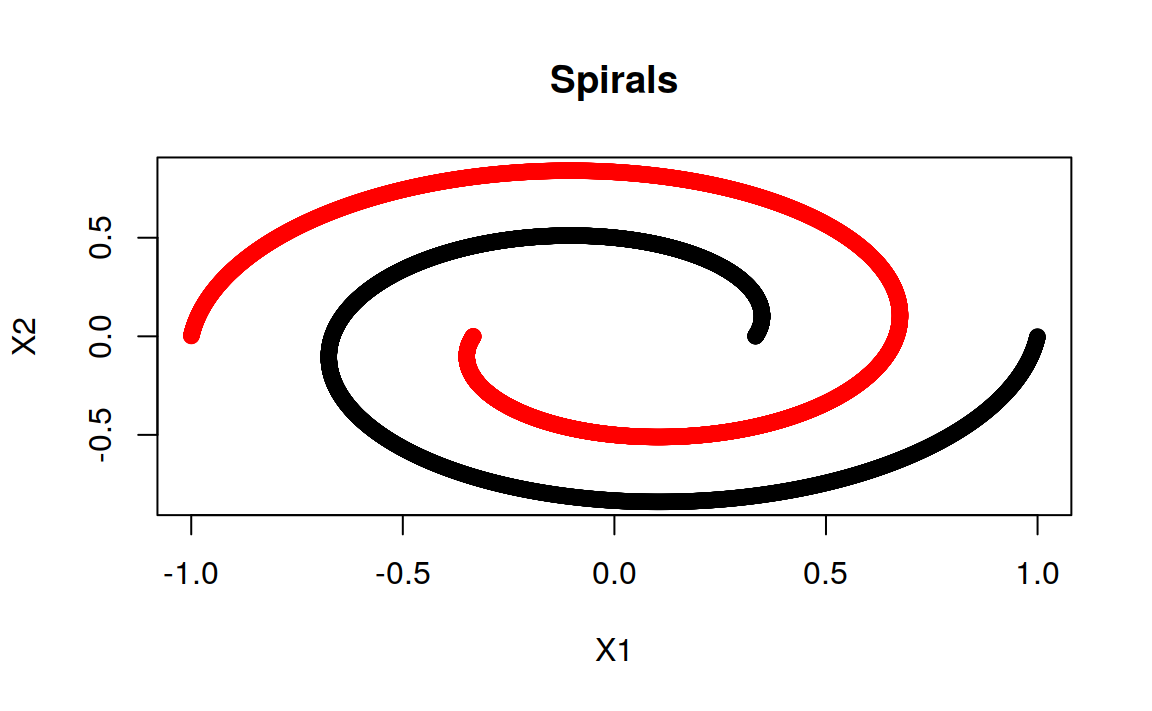
\includegraphics[width=0.7\linewidth]{neural_networks_from_scratch-examples-202d_files/figure-latex/load_mlbench-1} \end{center}

\begin{Shaded}
\begin{Highlighting}[]
\CommentTok{# Let's use all of this data for training}
\NormalTok{training_data <-}\StringTok{ }\KeywordTok{train_test_from_df}\NormalTok{(}\DataTypeTok{df =}\NormalTok{ data_df, }\DataTypeTok{predict_col_index =} \DecValTok{3}\NormalTok{, }
                                    \DataTypeTok{train_ratio =} \DecValTok{1}\NormalTok{, }\DataTypeTok{scale_input =} \OtherTok{TRUE}\NormalTok{)[[}\DecValTok{1}\NormalTok{]]}
\NormalTok{in_n <-}\StringTok{ }\KeywordTok{length}\NormalTok{(training_data[[}\DecValTok{1}\NormalTok{]][[}\DecValTok{1}\NormalTok{]])}
\NormalTok{out_n <-}\StringTok{ }\KeywordTok{length}\NormalTok{(training_data[[}\DecValTok{1}\NormalTok{]][[}\OperatorTok{-}\DecValTok{1}\NormalTok{]])}
\end{Highlighting}
\end{Shaded}

\begin{Shaded}
\begin{Highlighting}[]
\CommentTok{# Wrap a function that trains a network and plots the classification}
\NormalTok{plotBoundaryLinePerNeuron <-}\StringTok{ }\ControlFlowTok{function}\NormalTok{(neurons, epochs)}
\NormalTok{\{}
\NormalTok{  trained_net <-}\StringTok{ }\KeywordTok{neuralnetwork}\NormalTok{(}\KeywordTok{c}\NormalTok{(in_n, neurons, out_n), training_data, }
\NormalTok{                               epochs, }\DecValTok{500}\NormalTok{, }\DecValTok{3}\NormalTok{, }\StringTok{'ce'}\NormalTok{)}
\NormalTok{  b <-}\StringTok{ }\NormalTok{trained_net[[}\DecValTok{1}\NormalTok{]]}
\NormalTok{  w <-}\StringTok{ }\NormalTok{trained_net[[}\OperatorTok{-}\DecValTok{1}\NormalTok{]]}
  \CommentTok{# Evaluate}
\NormalTok{  confusion <-}\StringTok{ }\KeywordTok{evaluate}\NormalTok{(training_data, b, w)}
  \CommentTok{# Generate new-data}
\NormalTok{  nd <-}\StringTok{ }\KeywordTok{as.data.frame}\NormalTok{(}\KeywordTok{matrix}\NormalTok{(}\KeywordTok{runif}\NormalTok{(}\DecValTok{100000}\NormalTok{, }\DataTypeTok{min=}\OperatorTok{-}\DecValTok{1}\NormalTok{, }\DataTypeTok{max=}\DecValTok{1}\NormalTok{), }\DataTypeTok{ncol=}\DecValTok{2}\NormalTok{))}
  \CommentTok{# Get predictions}
\NormalTok{  nd}\OperatorTok{$}\NormalTok{res <-}\StringTok{ }\KeywordTok{as.factor}\NormalTok{(}\KeywordTok{unlist}\NormalTok{(}\KeywordTok{get_predictions}\NormalTok{(}\KeywordTok{as.list}\NormalTok{(}\KeywordTok{as.data.frame}\NormalTok{(}\KeywordTok{t}\NormalTok{(nd))), b, w)))}
  \CommentTok{# Plot predictions}
  \KeywordTok{plot}\NormalTok{(}\DataTypeTok{x=}\NormalTok{nd[,}\DecValTok{1}\NormalTok{], }\DataTypeTok{y=}\NormalTok{nd[,}\DecValTok{2}\NormalTok{], }\DataTypeTok{pch=}\DecValTok{19}\NormalTok{, }\DataTypeTok{col=}\NormalTok{nd[,}\DecValTok{3}\NormalTok{],}
       \DataTypeTok{main =} \KeywordTok{paste0}\NormalTok{(}\StringTok{"Spiral Boundary Line - "}\NormalTok{, neurons, }\StringTok{" neurons"}\NormalTok{), }
       \DataTypeTok{xlab =} \StringTok{"X1"}\NormalTok{, }\DataTypeTok{ylab =} \StringTok{"X2"}\NormalTok{)}
  \CommentTok{# Original points}
  \KeywordTok{points}\NormalTok{(}\DataTypeTok{x=}\NormalTok{data_df[,}\DecValTok{1}\NormalTok{], }\DataTypeTok{y=}\NormalTok{data_df[,}\DecValTok{2}\NormalTok{], }\DataTypeTok{pch=}\DecValTok{19}\NormalTok{, }\DataTypeTok{col=}\KeywordTok{ifelse}\NormalTok{(data_df[,}\DecValTok{3}\NormalTok{]}\OperatorTok{==}\DecValTok{2}\NormalTok{, }
                                                          \StringTok{"orange"}\NormalTok{, }\StringTok{"grey"}\NormalTok{))}
\NormalTok{\}}
\end{Highlighting}
\end{Shaded}

\begin{Shaded}
\begin{Highlighting}[]
 \KeywordTok{plotBoundaryLinePerNeuron}\NormalTok{(}\DecValTok{50}\NormalTok{, }\DecValTok{80}\NormalTok{)}
\CommentTok{#> Training complete[1] 1}
\end{Highlighting}
\end{Shaded}

\begin{center}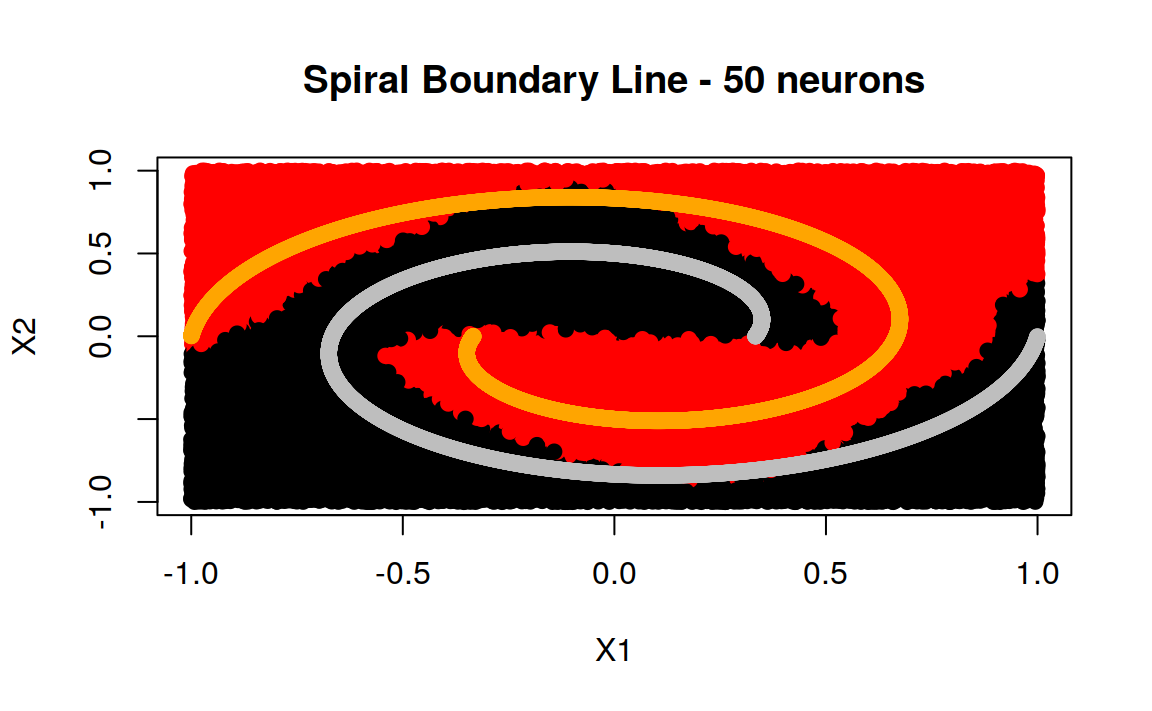
\includegraphics[width=0.7\linewidth]{neural_networks_from_scratch-examples-202d_files/figure-latex/spiral_n50_e80-1} \end{center}

\begin{Shaded}
\begin{Highlighting}[]
\CommentTok{# plotBoundaryLinePerNeuron(10, 80)}
\end{Highlighting}
\end{Shaded}

\begin{Shaded}
\begin{Highlighting}[]
\CommentTok{# plotBoundaryLinePerNeuron(5, 100)}
\end{Highlighting}
\end{Shaded}

\begin{Shaded}
\begin{Highlighting}[]
 \KeywordTok{plotBoundaryLinePerNeuron}\NormalTok{(}\DecValTok{4}\NormalTok{, }\DecValTok{100}\NormalTok{)}
\CommentTok{#> Training complete[1] 0.877}
\end{Highlighting}
\end{Shaded}

\begin{center}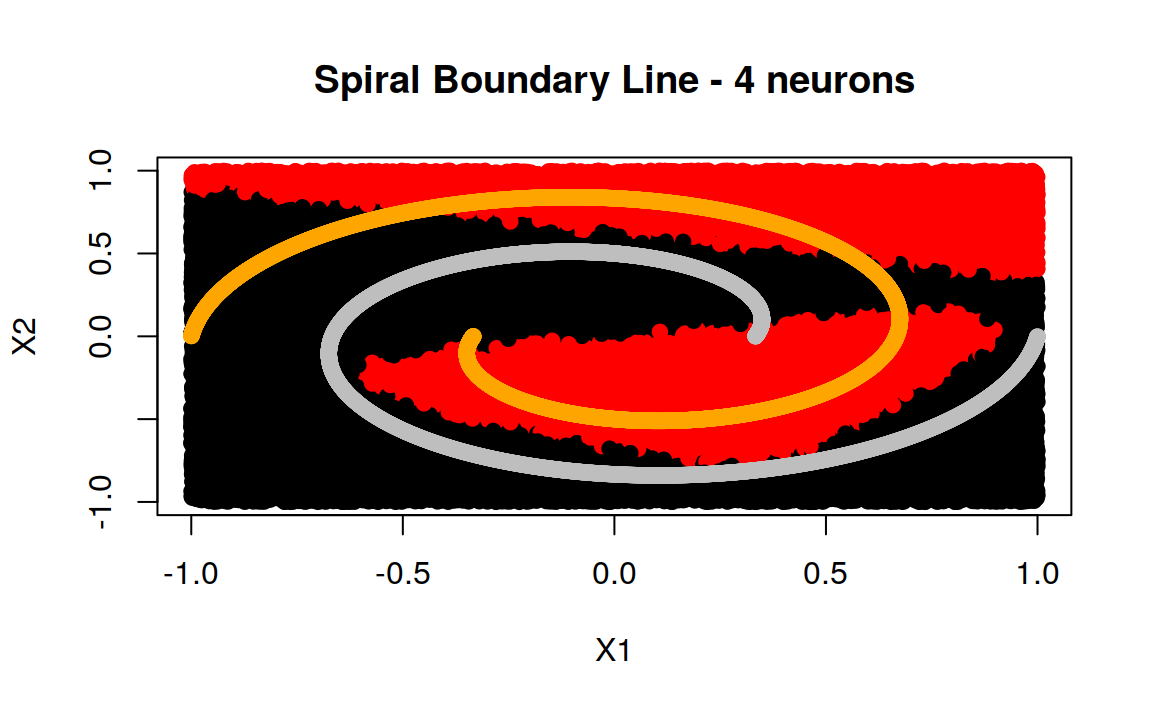
\includegraphics[width=0.7\linewidth]{neural_networks_from_scratch-examples-202d_files/figure-latex/spiral_n4_e100-1} \end{center}

It doesn't seem possible to draw fewer than 4 curves that split the classes, hence below 4 neurons we should start to see performance degrade - because the network doesn't enough params to fit the data. This can be a useful to exercise when trying to figure out how many neurons ones needs over-fitting

\begin{Shaded}
\begin{Highlighting}[]
 \KeywordTok{plotBoundaryLinePerNeuron}\NormalTok{(}\DecValTok{3}\NormalTok{, }\DecValTok{120}\NormalTok{)}
\CommentTok{#> Training complete[1] 0.786}
\end{Highlighting}
\end{Shaded}

\begin{center}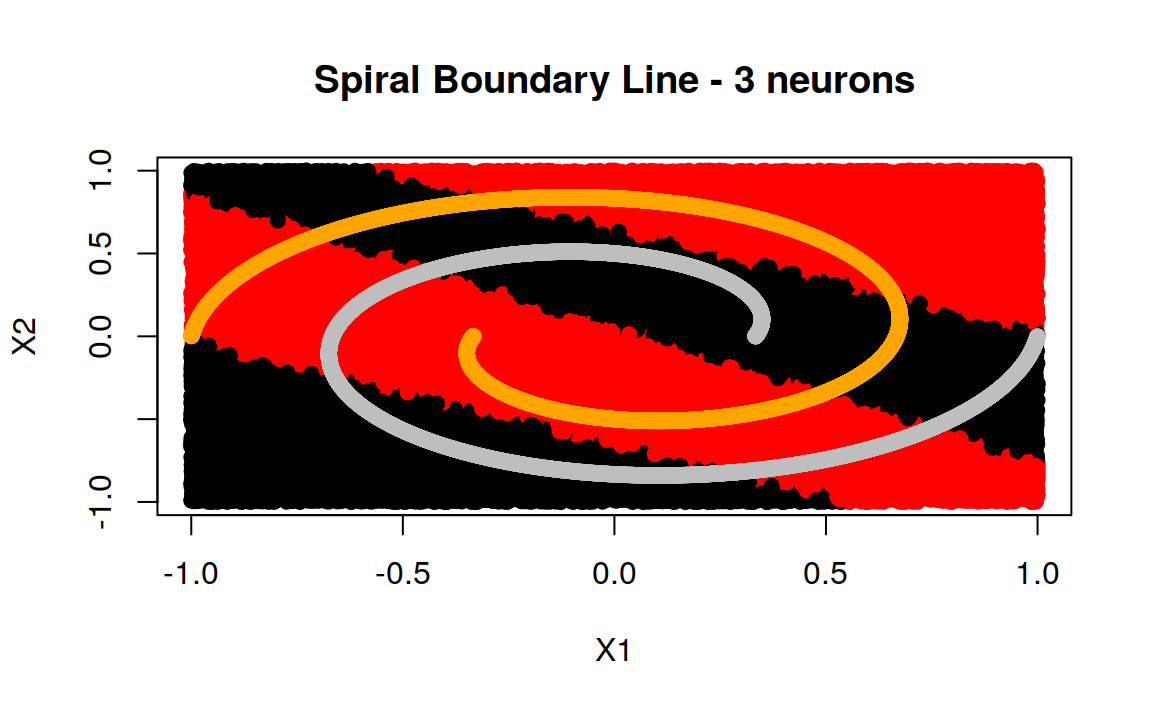
\includegraphics[width=0.7\linewidth]{neural_networks_from_scratch-examples-202d_files/figure-latex/spiral_n3_e120-1} \end{center}

\begin{Shaded}
\begin{Highlighting}[]
\CommentTok{# plotBoundaryLinePerNeuron(2, 200)}
\end{Highlighting}
\end{Shaded}

\begin{Shaded}
\begin{Highlighting}[]
\CommentTok{# plotBoundaryLinePerNeuron(1, 120)}
\end{Highlighting}
\end{Shaded}

\begin{Shaded}
\begin{Highlighting}[]
\CommentTok{# plotBoundaryLinePerNeuron(c(40,40,40), 200)}
\end{Highlighting}
\end{Shaded}

\hypertarget{what-is-a-neural-network}{%
\section{What is a neural network?}\label{what-is-a-neural-network}}

A neural network can be thought of as a series of logistic regressions stacked on top of each other. This means we could say that a logistic regression is a neural-network (with sigmoid activations) with no hidden-layer.

This hidden-layer lets a neural-network generate non-linearities and leads to the Universal approximation theorem, which states that a network with just one hidden layer can approximate any linear or non-linear function. The number of hidden-layers can go into the hundreds.

It can be useful to think of a neural-network as a combination of two things: 1) many logistic regressions stacked on top of each other that are `feature-generators' and 2) one read-out-layer which is just a softmax regression. The recent successes in deep-learning can arguable be attributed to the `feature-generators'. For example; previously with computer vision, we had to painfully state that we wanted to find triangles, circles, colours, and in what combination (similar to how economists decide which interaction-terms they need in a linear regression). Now, the hidden-layers are basically an optimisation to decide which features (which `interaction-terms') to extract. A lot of deep-learning (transfer learning) is actually done by generating features using a trained-model with the head (read-out layer) cut-off, and then training a logistic regression (or boosted decision-trees) using those features as inputs.

The hidden-layer also means that our loss function is not convex in parameters and we can't roll down a smooth-hill to get to the bottom. Instead of using Gradient Descent (which we did for the case of a logistic-regression) we will use Stochastic Gradient Descent (SGD), which basically shuffles the observations (random/stochastic) and updates the gradient after each mini-batch (generally much less than total number of observations) has been propagated through the network. There are many alternatives to SGD that Sebastian Ruder does a great job of summarising here. I think this is a fascinating topic to go through, but outside the scope of this blog-post. Briefly, however, the vast majority of the optimisation methods are first-order (including SGD, Adam, RMSprop, and Adagrad) because calculating the second-order is too computionally difficult. However, some of these first-order methods have a fixed learning-rate (SGD) and some have an adaptive learning-rate (Adam), which means that the `amount' we update our weights by becomes a function of the loss - we may make big jumps in the beginning but then take smaller steps as we get closer to the target.

It should be clear, however that minimising the loss on training data is not the main goal - in theory we want to minimise the loss on `unseen'/test data; hence all the opimisation methods proxy for that under the assumption that a low lost on training data will generalise to `new' data from the same distribution. This means we may prefer a neural-network with a higher training-loss; because it has a lower validation-loss (on data it hasn't been trained on) - we would typically say that the network has `overfit' in this case. There have been some recent papers that claim that adaptive optimisation methods do not generalise as well as SGD because they find very sharp minima points.

Previously we only had to back-propagate the gradient one layer, now we also have to back-propagate it through all the hidden-layers. Explaining the back-propagation algorithm is beyond the scope of this post, however it is crucial to understand. Many good resources exist online to help.

We can now create a neural-network from scratch in R using four functions.

First, we initialise our weights:

\begin{Shaded}
\begin{Highlighting}[]
\NormalTok{neuralnetwork <-}\StringTok{ }\ControlFlowTok{function}\NormalTok{(sizes, training_data, epochs, }
\NormalTok{  mini_batch_size, lr, C, }\DataTypeTok{verbose=}\OtherTok{FALSE}\NormalTok{, }
  \DataTypeTok{validation_data=}\NormalTok{training_data)}
\end{Highlighting}
\end{Shaded}

Since we now have a complex combination of parameters we can't just initialise them to be 1 or 0, like before - the network may get stuck. To help, we use the gaussian distribution (however, just like with the opimisation, there are many other methods):

\begin{Shaded}
\begin{Highlighting}[]
\NormalTok{    biases <-}\StringTok{ }\KeywordTok{lapply}\NormalTok{(}\KeywordTok{seq_along}\NormalTok{(listb), }\ControlFlowTok{function}\NormalTok{(idx)\{}
\NormalTok{    r <-}\StringTok{ }\NormalTok{listb[[idx]]}
    \KeywordTok{matrix}\NormalTok{(}\KeywordTok{rnorm}\NormalTok{(}\DataTypeTok{n=}\NormalTok{r), }\DataTypeTok{nrow=}\NormalTok{r, }\DataTypeTok{ncol=}\DecValTok{1}\NormalTok{)}
\NormalTok{    \})}

\NormalTok{    weights <-}\StringTok{ }\KeywordTok{lapply}\NormalTok{(}\KeywordTok{seq_along}\NormalTok{(listb), }\ControlFlowTok{function}\NormalTok{(idx)\{}
\NormalTok{    c <-}\StringTok{ }\NormalTok{listw[[idx]]}
\NormalTok{    r <-}\StringTok{ }\NormalTok{listb[[idx]]}
    \KeywordTok{matrix}\NormalTok{(}\KeywordTok{rnorm}\NormalTok{(}\DataTypeTok{n=}\NormalTok{r}\OperatorTok{*}\NormalTok{c), }\DataTypeTok{nrow=}\NormalTok{r, }\DataTypeTok{ncol=}\NormalTok{c)}
\NormalTok{    \})}
\end{Highlighting}
\end{Shaded}

Second, we use stochastic gradient descent as our optimisation method:

\begin{Shaded}
\begin{Highlighting}[]
\NormalTok{SGD <-}\StringTok{ }\ControlFlowTok{function}\NormalTok{(training_data, epochs, mini_batch_size, lr, C, sizes, }
\NormalTok{                num_layers, biases, weights,}
                 \DataTypeTok{verbose=}\OtherTok{FALSE}\NormalTok{, validation_data)}
\NormalTok{ \{}
   \CommentTok{# Every epoch}
   \ControlFlowTok{for}\NormalTok{ (j }\ControlFlowTok{in} \DecValTok{1}\OperatorTok{:}\NormalTok{epochs)\{}
     \CommentTok{# Stochastic mini-batch (shuffle data)}
\NormalTok{     training_data <-}\StringTok{ }\KeywordTok{sample}\NormalTok{(training_data)}
     \CommentTok{# Partition set into mini-batches}
\NormalTok{     mini_batches <-}\StringTok{ }\KeywordTok{split}\NormalTok{(training_data, }
                           \KeywordTok{ceiling}\NormalTok{(}\KeywordTok{seq_along}\NormalTok{(training_data)}\OperatorTok{/}\NormalTok{mini_batch_size))}
     \CommentTok{# Feed forward (and back) all mini-batches}
     \ControlFlowTok{for}\NormalTok{ (k }\ControlFlowTok{in} \DecValTok{1}\OperatorTok{:}\KeywordTok{length}\NormalTok{(mini_batches)) \{}
       \CommentTok{# Update biases and weights}
\NormalTok{       res <-}\StringTok{ }\KeywordTok{update_mini_batch}\NormalTok{(mini_batches[[k]], lr, C, sizes, num_layers, biases, weights)}
\NormalTok{       biases <-}\StringTok{ }\NormalTok{res[[}\DecValTok{1}\NormalTok{]]}
\NormalTok{       weights <-}\StringTok{ }\NormalTok{res[[}\OperatorTok{-}\DecValTok{1}\NormalTok{]]}
\NormalTok{     \}}
\NormalTok{   \}}
   \CommentTok{# Return trained biases and weights}
   \KeywordTok{list}\NormalTok{(biases, weights)}
\NormalTok{ \}}
\end{Highlighting}
\end{Shaded}

Third, as part of the SGD method, we update the weights after each mini-batch has been forward and backwards-propagated:

\begin{Shaded}
\begin{Highlighting}[]
\NormalTok{update_mini_batch <-}\StringTok{ }\ControlFlowTok{function}\NormalTok{(mini_batch, lr, C, sizes, num_layers, biases, weights)}
\NormalTok{ \{}
\NormalTok{   nmb <-}\StringTok{ }\KeywordTok{length}\NormalTok{(mini_batch)}
\NormalTok{   listw <-}\StringTok{ }\NormalTok{sizes[}\DecValTok{1}\OperatorTok{:}\KeywordTok{length}\NormalTok{(sizes)}\OperatorTok{-}\DecValTok{1}\NormalTok{] }
\NormalTok{   listb <-}\StringTok{  }\NormalTok{sizes[}\OperatorTok{-}\DecValTok{1}\NormalTok{]  }

   \CommentTok{# Initialise updates with zero vectors (for EACH mini-batch)}
\NormalTok{   nabla_b <-}\StringTok{ }\KeywordTok{lapply}\NormalTok{(}\KeywordTok{seq_along}\NormalTok{(listb), }\ControlFlowTok{function}\NormalTok{(idx)\{}
\NormalTok{     r <-}\StringTok{ }\NormalTok{listb[[idx]]}
     \KeywordTok{matrix}\NormalTok{(}\DecValTok{0}\NormalTok{, }\DataTypeTok{nrow=}\NormalTok{r, }\DataTypeTok{ncol=}\DecValTok{1}\NormalTok{)}
\NormalTok{   \})}
\NormalTok{   nabla_w <-}\StringTok{ }\KeywordTok{lapply}\NormalTok{(}\KeywordTok{seq_along}\NormalTok{(listb), }\ControlFlowTok{function}\NormalTok{(idx)\{}
\NormalTok{     c <-}\StringTok{ }\NormalTok{listw[[idx]]}
\NormalTok{     r <-}\StringTok{ }\NormalTok{listb[[idx]]}
     \KeywordTok{matrix}\NormalTok{(}\DecValTok{0}\NormalTok{, }\DataTypeTok{nrow=}\NormalTok{r, }\DataTypeTok{ncol=}\NormalTok{c)}
\NormalTok{   \})  }

   \CommentTok{# Go through mini_batch}
   \ControlFlowTok{for}\NormalTok{ (i }\ControlFlowTok{in} \DecValTok{1}\OperatorTok{:}\NormalTok{nmb)\{}
\NormalTok{     x <-}\StringTok{ }\NormalTok{mini_batch[[i]][[}\DecValTok{1}\NormalTok{]]}
\NormalTok{     y <-}\StringTok{ }\NormalTok{mini_batch[[i]][[}\OperatorTok{-}\DecValTok{1}\NormalTok{]]}
     \CommentTok{# Back propogation will return delta}
     \CommentTok{# Backprop for each observation in mini-batch}
\NormalTok{     delta_nablas <-}\StringTok{ }\KeywordTok{backprop}\NormalTok{(x, y, C, sizes, num_layers, biases, weights)}
\NormalTok{     delta_nabla_b <-}\StringTok{ }\NormalTok{delta_nablas[[}\DecValTok{1}\NormalTok{]]}
\NormalTok{     delta_nabla_w <-}\StringTok{ }\NormalTok{delta_nablas[[}\OperatorTok{-}\DecValTok{1}\NormalTok{]]}
     \CommentTok{# Add on deltas to nabla}
\NormalTok{     nabla_b <-}\StringTok{ }\KeywordTok{lapply}\NormalTok{(}\KeywordTok{seq_along}\NormalTok{(biases),}\ControlFlowTok{function}\NormalTok{(j)}
       \KeywordTok{unlist}\NormalTok{(nabla_b[[j]])}\OperatorTok{+}\KeywordTok{unlist}\NormalTok{(delta_nabla_b[[j]]))}
\NormalTok{     nabla_w <-}\StringTok{ }\KeywordTok{lapply}\NormalTok{(}\KeywordTok{seq_along}\NormalTok{(weights),}\ControlFlowTok{function}\NormalTok{(j)}
       \KeywordTok{unlist}\NormalTok{(nabla_w[[j]])}\OperatorTok{+}\KeywordTok{unlist}\NormalTok{(delta_nabla_w[[j]]))}
\NormalTok{   \}}
   \CommentTok{# After mini-batch has finished update biases and weights:}
   \CommentTok{# i.e. weights = weights - (learning-rate/numbr in batch)*nabla_weights}
   \CommentTok{# Opposite direction of gradient}
\NormalTok{   weights <-}\StringTok{ }\KeywordTok{lapply}\NormalTok{(}\KeywordTok{seq_along}\NormalTok{(weights), }\ControlFlowTok{function}\NormalTok{(j)}
     \KeywordTok{unlist}\NormalTok{(weights[[j]])}\OperatorTok{-}\NormalTok{(lr}\OperatorTok{/}\NormalTok{nmb)}\OperatorTok{*}\KeywordTok{unlist}\NormalTok{(nabla_w[[j]]))}
\NormalTok{   biases <-}\StringTok{ }\KeywordTok{lapply}\NormalTok{(}\KeywordTok{seq_along}\NormalTok{(biases), }\ControlFlowTok{function}\NormalTok{(j)}
     \KeywordTok{unlist}\NormalTok{(biases[[j]])}\OperatorTok{-}\NormalTok{(lr}\OperatorTok{/}\NormalTok{nmb)}\OperatorTok{*}\KeywordTok{unlist}\NormalTok{(nabla_b[[j]]))}
   \CommentTok{# Return}
   \KeywordTok{list}\NormalTok{(biases, weights)}
\NormalTok{ \}}
\end{Highlighting}
\end{Shaded}

Fourth, the algorithm we use to calculate the deltas is the back-propagation algorithm.

In this example we use the cross-entropy loss function, which produces the following gradient:

\begin{Shaded}
\begin{Highlighting}[]
\NormalTok{cost_delta <-}\StringTok{ }\ControlFlowTok{function}\NormalTok{(method, z, a, y) \{}
  \ControlFlowTok{if}\NormalTok{ (method}\OperatorTok{==}\StringTok{'ce'}\NormalTok{)\{}\KeywordTok{return}\NormalTok{ (a}\OperatorTok{-}\NormalTok{y)\}}
\NormalTok{\}}
\end{Highlighting}
\end{Shaded}

Also, to be consistent with our logistic regression example we use the sigmoid activation for the hidden layers and for the read-out layer:

\begin{Shaded}
\begin{Highlighting}[]
\CommentTok{# Calculate activation function}
\NormalTok{sigmoid <-}\StringTok{ }\ControlFlowTok{function}\NormalTok{(z)\{}\FloatTok{1.0}\OperatorTok{/}\NormalTok{(}\FloatTok{1.0}\OperatorTok{+}\KeywordTok{exp}\NormalTok{(}\OperatorTok{-}\NormalTok{z))\}}
\CommentTok{# Partial derivative of activation function}
\NormalTok{sigmoid_prime <-}\StringTok{ }\ControlFlowTok{function}\NormalTok{(z)\{}\KeywordTok{sigmoid}\NormalTok{(z)}\OperatorTok{*}\NormalTok{(}\DecValTok{1}\OperatorTok{-}\KeywordTok{sigmoid}\NormalTok{(z))\}}
\end{Highlighting}
\end{Shaded}

As mentioned previously, usually the softmax activation is used for the read-out layer. For the hidden layers, ReLU is more common, which is just the max function (negative weights get flattened to 0). The activation function for the hidden layers can be imagined as a race to carry a baton/flame (gradient) without it dying. The sigmoid function flattens out at 0 and at 1, resulting in a flat gradient which is equivalent to the flame dying out (we have lost our signal). The ReLU function helps preserve this gradient.

The back-propagation function is defined as:

\begin{Shaded}
\begin{Highlighting}[]
\NormalTok{backprop <-}\StringTok{ }\ControlFlowTok{function}\NormalTok{(x, y, C, sizes, num_layers, biases, weights)}
\end{Highlighting}
\end{Shaded}

Check out the notebook for the full code --- however the principle remains the same: we have a forward-pass where we generate our prediction by propagating the weights through all the layers of the network. We then plug this into the cost gradient and update the weights through all of our layers.

This concludes the creation of a neural network (with as many hidden layers as you desire). It can be a good exercise to replace the hidden-layer activation with ReLU and read-out to be softmax, and also add L1 and L2 regularization. Running this on the iris dataset in the notebook (which contains 4 explanatory variables with 3 possible outomes), with just one hidden-layer containing 40 neurons we get an accuracy of 96\% after 30 rounds/epochs of training.

The notebook also runs a 100-neuron handwriting-recognition example to predict the digit corresponding to a 28x28 pixel image.

\hypertarget{logistic-regression}{%
\chapter{Logistic Regression}\label{logistic-regression}}

\url{https://github.com/ilkarman/DemoNeuralNet/blob/master/02_LogisticRegression.ipynb}

\begin{Shaded}
\begin{Highlighting}[]
\NormalTok{knitr}\OperatorTok{::}\KeywordTok{include_graphics}\NormalTok{(}\KeywordTok{file.path}\NormalTok{(assets_dir, }\StringTok{"softmax_regression.jpg"}\NormalTok{))}
\end{Highlighting}
\end{Shaded}

\begin{center}\includegraphics[width=0.7\linewidth]{/home/datascience/repos/machine-learning-rsuite/import/assets/softmax_regression} \end{center}

\begin{Shaded}
\begin{Highlighting}[]
\NormalTok{knitr}\OperatorTok{::}\KeywordTok{include_graphics}\NormalTok{(}\KeywordTok{file.path}\NormalTok{(assets_dir, }\StringTok{"logistic_regression.jpg"}\NormalTok{))}
\end{Highlighting}
\end{Shaded}

\begin{center}\includegraphics[width=0.7\linewidth]{/home/datascience/repos/machine-learning-rsuite/import/assets/logistic_regression} \end{center}

\hypertarget{generate-the-data}{%
\section{Generate the data}\label{generate-the-data}}

\begin{Shaded}
\begin{Highlighting}[]
\CommentTok{# Reproduce results}
\KeywordTok{set.seed}\NormalTok{(}\DecValTok{1234567}\NormalTok{)}

\CommentTok{# Two possible outcomes -> binomial}
\NormalTok{data_df <-}\StringTok{ }\KeywordTok{as.data.frame}\NormalTok{(iris)}
\NormalTok{idx <-}\StringTok{ }\NormalTok{data_df}\OperatorTok{$}\NormalTok{Species }\OperatorTok\StringTok{ }\KeywordTok{c}\NormalTok{(}\StringTok{"virginica"}\NormalTok{, }\StringTok{"versicolor"}\NormalTok{)}
\NormalTok{data_df <-}\StringTok{ }\NormalTok{data_df[idx,]}
\NormalTok{y <-}\StringTok{ }\KeywordTok{ifelse}\NormalTok{(data_df}\OperatorTok{$}\NormalTok{Species}\OperatorTok{==}\StringTok{"virginica"}\NormalTok{, }\DecValTok{1}\NormalTok{, }\DecValTok{0}\NormalTok{)}

\CommentTok{# For faster convergence let's rescale X}
\CommentTok{# So that we can plot this consider only 2 variables}
\NormalTok{X <-}\StringTok{ }\NormalTok{data_df[}\KeywordTok{c}\NormalTok{(}\DecValTok{1}\NormalTok{,}\DecValTok{3}\NormalTok{)]}
\NormalTok{X <-}\StringTok{ }\KeywordTok{as.matrix}\NormalTok{(X}\OperatorTok{/}\KeywordTok{max}\NormalTok{(X))}

\CommentTok{# Resulting data-set}
\KeywordTok{head}\NormalTok{(X)}
\CommentTok{#>    Sepal.Length Petal.Length}
\CommentTok{#> 51        0.886        0.595}
\CommentTok{#> 52        0.810        0.570}
\CommentTok{#> 53        0.873        0.620}
\CommentTok{#> 54        0.696        0.506}
\CommentTok{#> 55        0.823        0.582}
\CommentTok{#> 56        0.722        0.570}
\KeywordTok{head}\NormalTok{(y)}
\CommentTok{#> [1] 0 0 0 0 0 0}
\end{Highlighting}
\end{Shaded}

\hypertarget{fit-a-binomial-logit-in-r}{%
\section{1. Fit a binomial logit in R}\label{fit-a-binomial-logit-in-r}}

A logistic regression is a linear regression that outputs a number bounded between 0 and 1. This means it is useful for classification problems, where we want to predict the probability of something happening. A binomial logistic regression is used when there are just two-classes, to extend beyound two-classes we would typically use a multi-nomial logistic regression (softmax).

Consider the iris-dataset where we try to predict whether a flower is ``virginica'' or ``versicolor'' by only looking at petal-length and sepal-length. We fit a linear line to `best' split the categories:

\begin{Shaded}
\begin{Highlighting}[]
\CommentTok{# Fit model}
\NormalTok{model <-}\StringTok{ }\KeywordTok{glm}\NormalTok{(y }\OperatorTok{~}\StringTok{ }\NormalTok{X, }\DataTypeTok{family=}\KeywordTok{binomial}\NormalTok{(}\DataTypeTok{link=}\StringTok{'logit'}\NormalTok{))}

\CommentTok{# Params}
\KeywordTok{print}\NormalTok{(}\KeywordTok{coef}\NormalTok{(model))}
\CommentTok{#>   (Intercept) XSepal.Length XPetal.Length }
\CommentTok{#>         -39.8         -31.7         105.2}
\CommentTok{# Coefficients:}
\CommentTok{# (Intercept) XSepal.Length XPetal.Length }
\CommentTok{# -39.83851     -31.73243     105.16992 }
\CommentTok{#summary(model)}

\CommentTok{# Visualise the decision boundary}
\NormalTok{intcp <-}\StringTok{ }\KeywordTok{coef}\NormalTok{(model)[}\DecValTok{1}\NormalTok{]}\OperatorTok{/-}\NormalTok{(}\KeywordTok{coef}\NormalTok{(model)[}\DecValTok{3}\NormalTok{])}
\NormalTok{slope <-}\StringTok{ }\KeywordTok{coef}\NormalTok{(model)[}\DecValTok{2}\NormalTok{]}\OperatorTok{/-}\NormalTok{(}\KeywordTok{coef}\NormalTok{(model)[}\DecValTok{3}\NormalTok{])}

\CommentTok{# Our points}
\KeywordTok{plot}\NormalTok{(}\DataTypeTok{x=}\NormalTok{X[,}\DecValTok{1}\NormalTok{], }\DataTypeTok{y=}\NormalTok{X[,}\DecValTok{2}\NormalTok{], }\DataTypeTok{cex =} \DecValTok{1}\NormalTok{, }\DataTypeTok{col=}\NormalTok{data_df}\OperatorTok{$}\NormalTok{Species,}
     \DataTypeTok{main =} \StringTok{"Iris type by length and width"}\NormalTok{, }
     \DataTypeTok{xlab =} \StringTok{"Sepal Length"}\NormalTok{, }\DataTypeTok{ylab =} \StringTok{"Petal Length"}\NormalTok{)}
\KeywordTok{legend}\NormalTok{(}\DataTypeTok{x=}\StringTok{'topright'}\NormalTok{, }\DataTypeTok{legend=}\KeywordTok{unique}\NormalTok{(data_df}\OperatorTok{$}\NormalTok{Species),}\DataTypeTok{col=}\KeywordTok{unique}\NormalTok{(data_df}\OperatorTok{$}\NormalTok{Species), }\DataTypeTok{pch=}\DecValTok{1}\NormalTok{)}
\CommentTok{# Decision boundary}
\KeywordTok{abline}\NormalTok{(intcp , slope, }\DataTypeTok{col=}\StringTok{'blue'}\NormalTok{)}
\end{Highlighting}
\end{Shaded}

\begin{center}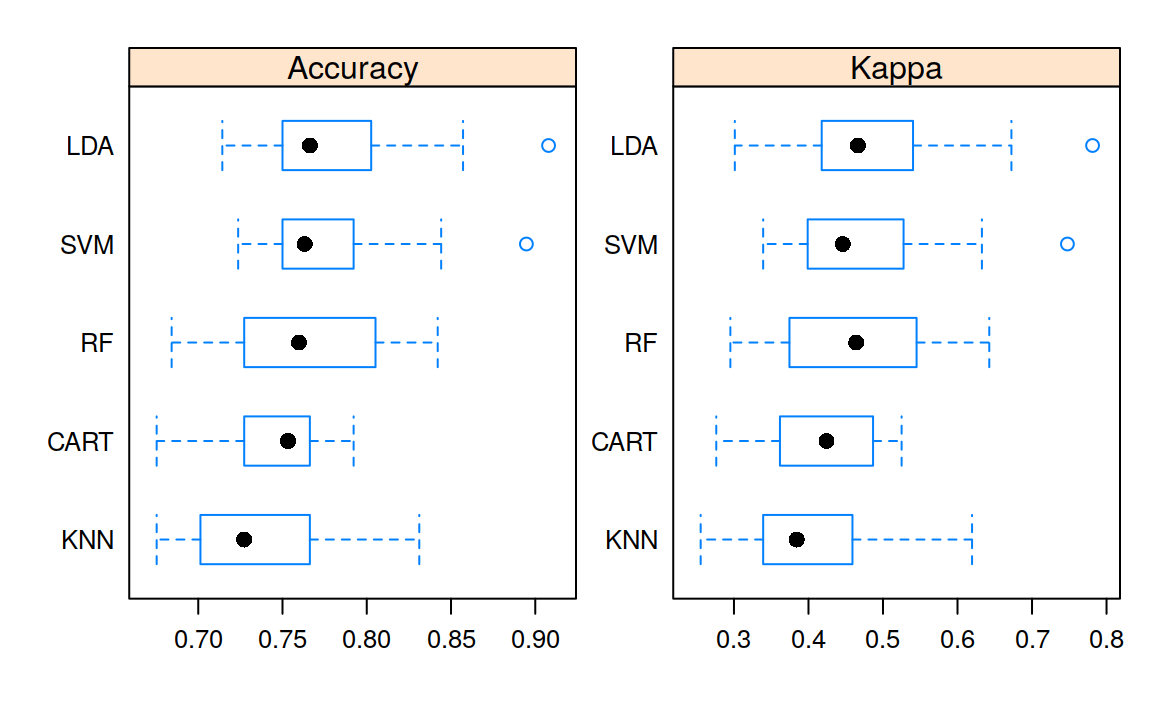
\includegraphics[width=0.7\linewidth]{neural_networks_from_scratch-logistic_regression-202b_files/figure-latex/unnamed-chunk-5-1} \end{center}

The above line has an intercept of -39.84, and coefficient of -31.73 for sepal-length and 105.17 for petal-length. These estimates are obtained by maximising the likelihood.

Because the log function is monotone, maximizing the likelihood is the same as maximizing the log-likelihood (or minimising the negative of the log-likelihood)

\[\begin{aligned} 
   l_x(\theta) = \log L_x(\theta)
\end{aligned}\]

For many reasons it is more convenient to use log likelihood rather than likelihood:

\[\begin{aligned}
   \log L_x
   =
   \sum_{i=1}^{N} y_i\beta^Tx_i - \log(1+e^{\beta^Tx_i})  
\end{aligned}\]

\begin{verbatim}
log_likelihood <- function(X_mat, y, beta_hat)
{
  scores <- X_mat %*% beta_hat
  ll <- (y * scores) - log(1+exp(scores))
  sum(ll)
}
\end{verbatim}

The log-likelihood in this example is -11.92.

\begin{Shaded}
\begin{Highlighting}[]
\KeywordTok{logLik}\NormalTok{(model)  }\CommentTok{# Log-likelihood}
\CommentTok{#> 'log Lik.' -11.9 (df=3)}

\CommentTok{# Calculate log-likelihood ourself}
\NormalTok{log_likelihood <-}\StringTok{ }\ControlFlowTok{function}\NormalTok{(X_mat, y, beta_hat)}
\NormalTok{\{}
\NormalTok{  scores <-}\StringTok{ }\NormalTok{X_mat }\OperatorTok\StringTok{ }\NormalTok{beta_hat}
  \CommentTok{# Need to broadcast (y %*% scores)}
\NormalTok{  ll <-}\StringTok{ }\NormalTok{(y }\OperatorTok{*}\StringTok{ }\NormalTok{scores) }\OperatorTok{-}\StringTok{ }\KeywordTok{log}\NormalTok{(}\DecValTok{1}\OperatorTok{+}\KeywordTok{exp}\NormalTok{(scores))}
  \KeywordTok{sum}\NormalTok{(ll)}
\NormalTok{\}}

\KeywordTok{log_likelihood}\NormalTok{(}\KeywordTok{cbind}\NormalTok{(}\DecValTok{1}\NormalTok{, X), y, }\KeywordTok{coef}\NormalTok{(model))  }\CommentTok{# Match at -11.925}
\CommentTok{#> [1] -11.9}
\end{Highlighting}
\end{Shaded}

\hypertarget{fit-a-binomial-logit-ourselves-gd}{%
\section{2. Fit a binomial logit ourselves (GD)}\label{fit-a-binomial-logit-ourselves-gd}}

Typically BFGS or other numerical optimisation procedures are used to minimise the cost/max log-likelihood instead of GD, because the parameter space is pretty smaller (compared to neural-networks).

The logistic loss is sometimes called the cross-entropy loss. Let us first examine what would happen if we simply tried to calculate the least-squares loss, like before (for a regression rather than a classification):

\[\begin{aligned} 
   C = \frac{1}{2n}\sum_x\|(y(x) - a(x)\|^2
\end{aligned}\]

This loss will not be convex (in parameters) because \(a(x)\) (the activation/link function) that transforms our score into a probability is defined as: \(\sigma(z)=\frac{1}{1+e^-z}\) and thus \(a(x)=\frac{1}{1+e^-\beta^Tx_i}\)

We can construct a convex-loss function. This is binary classification and so we can define the loss for both of the classes. When \(y=1\) we want the loss to be large when \(\sigma(z)\) is close to zero and for it to be small when it is close to 1. Similarly, when \(y=0\) we want the loss to be large when \(\sigma(z)\) is close to one and for it be small when it is close to 0. The following loss function satisifies those conditions:

\[\begin{aligned} 
   C = -\frac{1}{n}\sum_xy(x)\ln(a(x)) + (1 - y(x))\ln(1-a(x))
\end{aligned}\]

For example, when \(y(x)=1\) our loss-function becomes \(C = -\frac{1}{n}\sum_x\ln(a(x))\), which is equal to 0 when \(a(x)=1\), otherwise it becomes very high.

Taking the derivative of this loss-function w.r.t to the parameters, it can be shown:

\[\begin{aligned} 
    \frac{dC}{d\beta_i} = \frac{1}{n}\sum_xx_i(a(x) - y)
\end{aligned}\]

Note that the cross-entropy loss is more generally defined as:

\[\begin{aligned} 
   C = -\frac{1}{n}\sum_x\sum_j y_j\ln(a_j)
\end{aligned}\]

For binary classifications where \(j=2\), under the condition that the categories are mutually-exclusive \(\sum_ja_j=1\) and that y is one-hot so that \(y1+y2=1\), we can re-write it as:

\[\begin{aligned} 
   C = -\frac{1}{n}\sum_xy_1\ln(a_1) + (1 - y_1)\ln(1-a_1)
\end{aligned}\]

Which is the same equation we first started with.

The process for using GD for a logistic regression is similar to that of a simple linear-regression. Since our loss is convex we can use either gradient-descent or stochastic-gradient descent; for now we will stick with the former.

\begin{Shaded}
\begin{Highlighting}[]
\CommentTok{# Calculate activation function (sigmoid for logit)}
\NormalTok{sigmoid <-}\StringTok{ }\ControlFlowTok{function}\NormalTok{(z)\{}\FloatTok{1.0}\OperatorTok{/}\NormalTok{(}\FloatTok{1.0}\OperatorTok{+}\KeywordTok{exp}\NormalTok{(}\OperatorTok{-}\NormalTok{z))\}}

\NormalTok{logistic_reg <-}\StringTok{ }\ControlFlowTok{function}\NormalTok{(X, y, epochs, lr)}
\NormalTok{\{}
\NormalTok{  X_mat <-}\StringTok{ }\KeywordTok{cbind}\NormalTok{(}\DecValTok{1}\NormalTok{, X)}
\NormalTok{  beta_hat <-}\StringTok{ }\KeywordTok{matrix}\NormalTok{(}\DecValTok{1}\NormalTok{, }\DataTypeTok{nrow=}\KeywordTok{ncol}\NormalTok{(X_mat))}
  \ControlFlowTok{for}\NormalTok{ (j }\ControlFlowTok{in} \DecValTok{1}\OperatorTok{:}\NormalTok{epochs)}
\NormalTok{  \{}
\NormalTok{    residual <-}\StringTok{ }\KeywordTok{sigmoid}\NormalTok{(X_mat }\OperatorTok\StringTok{ }\NormalTok{beta_hat) }\OperatorTok{-}\StringTok{ }\NormalTok{y}
    \CommentTok{# Update weights with gradient descent}
\NormalTok{    delta <-}\StringTok{ }\KeywordTok{t}\NormalTok{(X_mat) }\OperatorTok\StringTok{ }\KeywordTok{as.matrix}\NormalTok{(residual, }\DataTypeTok{ncol=}\KeywordTok{nrow}\NormalTok{(X_mat)) }\OperatorTok{*}\StringTok{  }\NormalTok{(}\DecValTok{1}\OperatorTok{/}\KeywordTok{nrow}\NormalTok{(X_mat))}
\NormalTok{    beta_hat <-}\StringTok{ }\NormalTok{beta_hat }\OperatorTok{-}\StringTok{ }\NormalTok{(lr}\OperatorTok{*}\NormalTok{delta)}
\NormalTok{  \}}
  \CommentTok{# Print log-likliehood}
  \KeywordTok{print}\NormalTok{(}\KeywordTok{log_likelihood}\NormalTok{(X_mat, y, beta_hat))}
  \CommentTok{# Return}
\NormalTok{  beta_hat}
\NormalTok{\}}
\end{Highlighting}
\end{Shaded}

The only major difference is that we apply a sigmoid function to our prediction - to turn it into a probability. Below we can see why: the output is bounded between 0 and 1.

The shape of the sigmoid curve also means that we can increase the speed of convergence by scaling the variables to be closer to 0 - where the gradient is high. Imagine our inputs have a value of 100 - this can create a very high error, however the gradient is nearly flat and thus the update to the coefficients will be tiny.

We run the below to optimise our logistic regression using GD:

\begin{verbatim}
beta_hat <- logistic_reg(X, y, 300000, 5)
\end{verbatim}

We match the original results with the coefficients: -38.84, -31.73, 105.17

\begin{Shaded}
\begin{Highlighting}[]
\CommentTok{# Why did scaling before help with convergence?}
\CommentTok{# Vanishing gradient}
\KeywordTok{curve}\NormalTok{(sigmoid, }\DecValTok{-10}\NormalTok{, }\DecValTok{10}\NormalTok{)}
\end{Highlighting}
\end{Shaded}

\begin{center}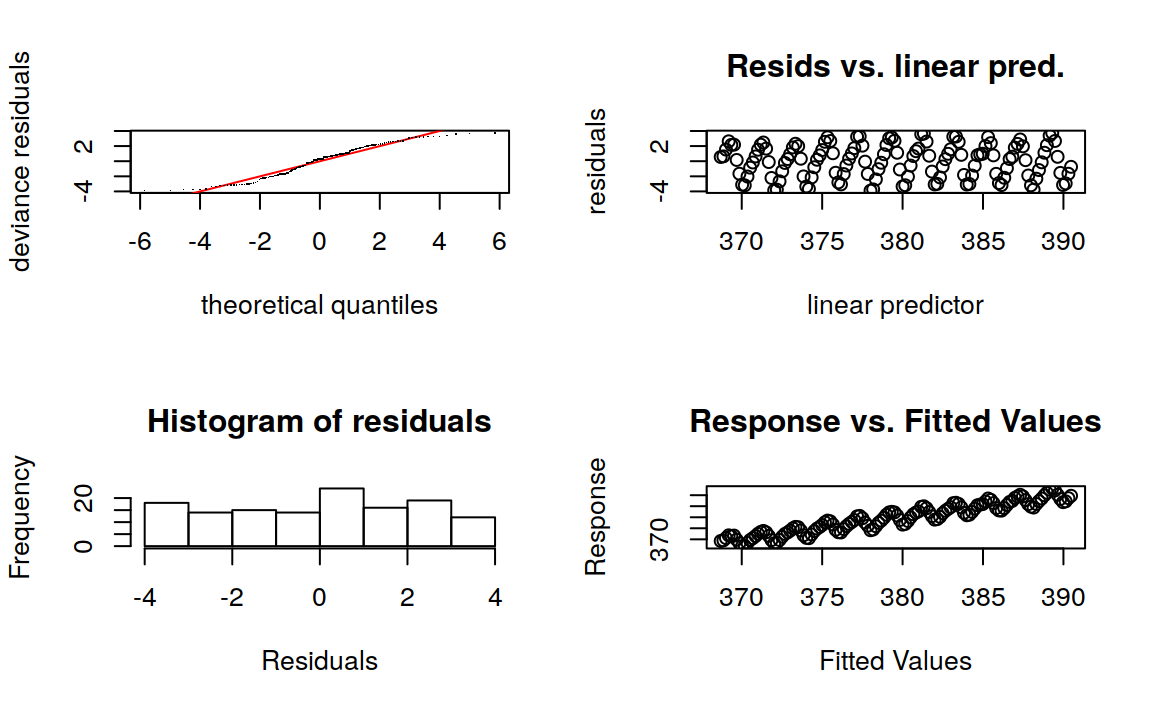
\includegraphics[width=0.7\linewidth]{neural_networks_from_scratch-logistic_regression-202b_files/figure-latex/unnamed-chunk-8-1} \end{center}

\begin{Shaded}
\begin{Highlighting}[]
\CommentTok{# Takes a while to converge with GD!}
\NormalTok{beta_hat <-}\StringTok{ }\KeywordTok{logistic_reg}\NormalTok{(X, y, }\DecValTok{300000}\NormalTok{, }\DecValTok{5}\NormalTok{)}
\CommentTok{#> [1] -11.9}
\KeywordTok{print}\NormalTok{(beta_hat)}
\CommentTok{#>               [,1]}
\CommentTok{#>              -39.8}
\CommentTok{#> Sepal.Length -31.7}
\CommentTok{#> Petal.Length 105.2}

\CommentTok{# Intercept    -39.83848}
\CommentTok{# Sepal.Length -31.73240}
\CommentTok{# Petal.Length 105.16983}

\CommentTok{# Visualise the decision boundary}
\KeywordTok{plot}\NormalTok{(}\DataTypeTok{x=}\NormalTok{X[,}\DecValTok{1}\NormalTok{], }\DataTypeTok{y=}\NormalTok{X[,}\DecValTok{2}\NormalTok{], }\DataTypeTok{cex =} \DecValTok{1}\NormalTok{, }\DataTypeTok{col=}\NormalTok{data_df}\OperatorTok{$}\NormalTok{Species,}
     \DataTypeTok{main =} \StringTok{"Iris type by length and width"}\NormalTok{, }
     \DataTypeTok{xlab =} \StringTok{"Sepal Length"}\NormalTok{, }\DataTypeTok{ylab =} \StringTok{"Petal Length"}\NormalTok{)}
\KeywordTok{legend}\NormalTok{(}\DataTypeTok{x=}\StringTok{'topright'}\NormalTok{, }\DataTypeTok{legend=}\KeywordTok{unique}\NormalTok{(data_df}\OperatorTok{$}\NormalTok{Species),}\DataTypeTok{col=}\KeywordTok{unique}\NormalTok{(data_df}\OperatorTok{$}\NormalTok{Species), }\DataTypeTok{pch=}\DecValTok{1}\NormalTok{)}

\CommentTok{# Visualise the decision boundary}
\NormalTok{intcp <-}\StringTok{ }\NormalTok{beta_hat[}\DecValTok{1}\NormalTok{]}\OperatorTok{/-}\NormalTok{(beta_hat[}\DecValTok{3}\NormalTok{])}
\NormalTok{slope <-}\StringTok{ }\NormalTok{beta_hat[}\DecValTok{2}\NormalTok{]}\OperatorTok{/-}\NormalTok{(beta_hat[}\DecValTok{3}\NormalTok{])}

\KeywordTok{abline}\NormalTok{(intcp , slope, }\DataTypeTok{col=}\StringTok{'purple'}\NormalTok{)}
\end{Highlighting}
\end{Shaded}

\begin{center}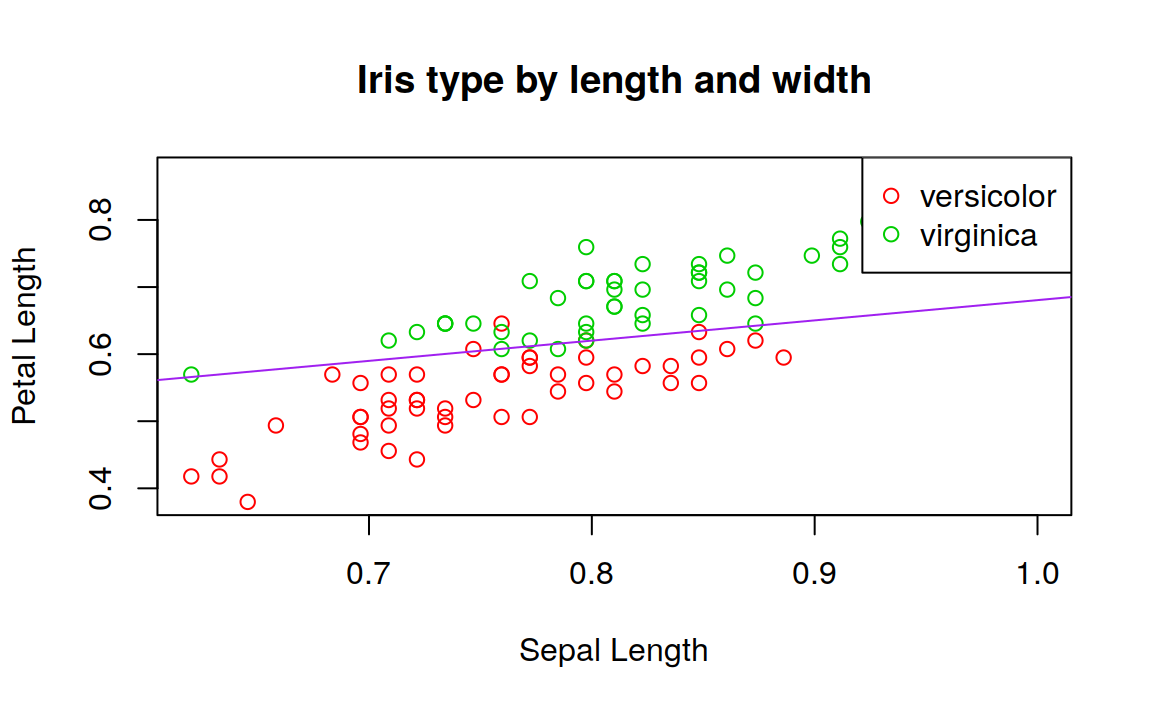
\includegraphics[width=0.7\linewidth]{neural_networks_from_scratch-logistic_regression-202b_files/figure-latex/logistic_gradient_descent-1} \end{center}

\hypertarget{what-is-logistic-regression}{%
\section{What is logistic regression?}\label{what-is-logistic-regression}}

A logistic regression is a linear regression for binary classification problems. The two main differences to a standard linear regression are:

We use an `activation'/link function called the logistic-sigmoid to squash the output to a probability bounded by 0 and 1
Instead of minimising the quadratic loss we minimise the negative log-likelihood of the Bernoulli distribution
Everything else remains the same.

We can calcuate our activation function like so:

\begin{Shaded}
\begin{Highlighting}[]
\NormalTok{sigmoid <-}\StringTok{ }\ControlFlowTok{function}\NormalTok{(z)\{}\FloatTok{1.0}\OperatorTok{/}\NormalTok{(}\FloatTok{1.0}\OperatorTok{+}\KeywordTok{exp}\NormalTok{(}\OperatorTok{-}\NormalTok{z))\}}
\end{Highlighting}
\end{Shaded}

We can create our log-likelihood function in R:

\begin{Shaded}
\begin{Highlighting}[]
\NormalTok{log_likelihood <-}\StringTok{ }\ControlFlowTok{function}\NormalTok{(X_mat, y, beta_hat)}
\NormalTok{\{}
\NormalTok{  scores <-}\StringTok{ }\NormalTok{X_mat }\OperatorTok\StringTok{ }\NormalTok{beta_hat}
\NormalTok{  ll <-}\StringTok{ }\NormalTok{(y }\OperatorTok{*}\StringTok{ }\NormalTok{scores) }\OperatorTok{-}\StringTok{ }\KeywordTok{log}\NormalTok{(}\DecValTok{1}\OperatorTok{+}\KeywordTok{exp}\NormalTok{(scores))}
  \KeywordTok{sum}\NormalTok{(ll)}
\NormalTok{\}}
\end{Highlighting}
\end{Shaded}

This loss function (the logistic loss or the log-loss) is also called the cross-entropy loss. The cross-entropy loss is basically a measure of `surprise' and will be the foundation for all the following models, so it is worth examining a bit more.

If we simply constructed the least-squares loss like before, because we now have a non-linear activation function (the sigmoid), the loss will no longer be convex which will make optimisation hard.

\[\begin{aligned} 
   C = \frac{1}{2n}\sum_x ((y(x) - a(x))^2
\end{aligned}\]

We could construct our own loss function for the two classes. When \(y=1\), we want our loss function to be very high if our prediction is close to 0, and very low when it is close to 1. When \(y=0\), we want our loss function to be very high if our prediction is close to 1, and very low when it is close to 0. This leads us to the following loss function:

\[\begin{aligned} 
   C = -\frac{1}{n}\sum_xy(x)\ln(a(x)) + (1 - y(x))\ln(1-a(x))
\end{aligned}\]

The delta for this loss function is pretty much the same as the one we had earlier for a linear-regression. The only difference is that we apply our sigmoid function to the prediction. This means that the GD function for a logistic regression will also look very similar:

\begin{Shaded}
\begin{Highlighting}[]
\NormalTok{logistic_reg <-}\StringTok{ }\ControlFlowTok{function}\NormalTok{(X, y, epochs, lr)}
\NormalTok{\{}
\NormalTok{  X_mat <-}\StringTok{ }\KeywordTok{cbind}\NormalTok{(}\DecValTok{1}\NormalTok{, X)}
\NormalTok{  beta_hat <-}\StringTok{ }\KeywordTok{matrix}\NormalTok{(}\DecValTok{1}\NormalTok{, }\DataTypeTok{nrow=}\KeywordTok{ncol}\NormalTok{(X_mat))}
  \ControlFlowTok{for}\NormalTok{ (j }\ControlFlowTok{in} \DecValTok{1}\OperatorTok{:}\NormalTok{epochs)}
\NormalTok{  \{}
    \CommentTok{# For a linear regression this was:}
    \CommentTok{# 1*(X_mat %*% beta_hat) - y}
\NormalTok{    residual <-}\StringTok{ }\KeywordTok{sigmoid}\NormalTok{(X_mat }\OperatorTok\StringTok{ }\NormalTok{beta_hat) }\OperatorTok{-}\StringTok{ }\NormalTok{y}
    \CommentTok{# Update weights with gradient descent}
\NormalTok{    delta <-}\StringTok{ }\KeywordTok{t}\NormalTok{(X_mat) }\OperatorTok\StringTok{ }\KeywordTok{as.matrix}\NormalTok{(residual, }\DataTypeTok{ncol=}\KeywordTok{nrow}\NormalTok{(X_mat))}\OperatorTok{*}\NormalTok{(}\DecValTok{1}\OperatorTok{/}\KeywordTok{nrow}\NormalTok{(X_mat))}
\NormalTok{    beta_hat <-}\StringTok{ }\NormalTok{beta_hat }\OperatorTok{-}\StringTok{ }\NormalTok{(lr}\OperatorTok{*}\NormalTok{delta)}
\NormalTok{  \}}
  \CommentTok{# Print log-likliehood}
  \KeywordTok{print}\NormalTok{(}\KeywordTok{log_likelihood}\NormalTok{(X_mat, y, beta_hat))}
  \CommentTok{# Return}
\NormalTok{  beta_hat}
\NormalTok{\}}
\end{Highlighting}
\end{Shaded}

\hypertarget{softmax-regression}{%
\section{Softmax Regression}\label{softmax-regression}}

\begin{Shaded}
\begin{Highlighting}[]
\NormalTok{knitr}\OperatorTok{::}\KeywordTok{include_graphics}\NormalTok{(}\KeywordTok{file.path}\NormalTok{(assets_dir, }\StringTok{"softmax_regression.jpg"}\NormalTok{))}
\end{Highlighting}
\end{Shaded}

\begin{center}\includegraphics[width=0.7\linewidth]{/home/datascience/repos/machine-learning-rsuite/import/assets/softmax_regression} \end{center}

A generalisation of the logistic regression is the multinomial logistic regression (also called `softmax'), which is used when there are more than two classes to predict. I haven't created this example in R, because the neural-network in the next step can reduce to something similar, however for completeness I wanted to highlight the main differences if you wanted to create it.

First, instead of using the sigmoid function to squash our (one) value between \(\theta\) and 1:

\[\sigma(z) = \frac {1}{1+e^{-z}}\]

We use the softmax function to squash the sum of our \(n\) values (for \(n\) classes) to 1:

\[\phi(z) = \frac {e^z_j}{\sum_k e^z_k}\]

This means the value supplied for each class can be interpreted as the probability of that class, given the evidence. This also means that when we see the target class and increase the weights to increase the probability of observing it, the probability of the other classes will fall. The implicit assumption is that our classes are mutually exclusive.

Second, we use a more general version of the cross-entropy loss function:

\[\begin{aligned} 
   C = -\frac{1}{n}\sum_x\sum_j y_j\ln(a_j)
\end{aligned}\]

To see why, remember that for binary classifications (previous example) we had two classes:
\(j=2\), under the condition that the categories are mutually-exclusive \(\sum_ja_j = 1\) and that \(y\) is one-hot so that \(y_1+y_2=1\), we can re-write the general formula as:

\[\begin{aligned} 
   C = -\frac{1}{n}\sum_xy_1\ln(a_1) + (1 - y_1)\ln(1-a_1)
\end{aligned}\]

Which is the same equation we first started with. However, now we relax the constraint that
\(j=2\). It can be shown that the cross-entropy loss here has the same gradient as for the case of the binary/two-class cross-entropy on logistic outputs.

\[\begin{aligned} 
   \frac {\partial C} {\partial \beta_i} = \frac {1}{n} \sum x_i(a(x) -y)
\end{aligned}\]

However, although the gradient has the same formula it will be different because the activation here takes on a different value (softmax instead of logistic-sigmoid).

In most deep-learning frameworks you have the choice of `binary-crossentropy' or `categorical-crossentropy' loss. Depending on whether your last layer contains sigmoid or softmax activation you would want to choose binary or categorical cross-entropy (respectively). The training of the network should not be affected, since the gradient is the same, however the reported loss (for evaluation) would be wrong if these are mixed up.

The motivation to go through softmax is that most neural-networks will use a softmax layer as the final/`read-out' layer, with a multinomial/categorical cross-entropy loss instead of using sigmoids with a binary cross-entropy loss --- when the categories are mutually exclusive. Although multiple sigmoids for multiple classes can also be used (and will be used in the next example), this is generally only used for the case of non-mutually-exclusive labels (i.e.~we can have multiple labels). With a softmax output, since the sum of the outputs is constrained to equal 1, we have the advantage of interpreting the outputs as class probabilities.

\hypertarget{neural-networks-what-is-it}{%
\chapter{Neural Networks: What is it?}\label{neural-networks-what-is-it}}

Source: \url{https://github.com/ilkarman/DemoNeuralNet/blob/master/03_NeuralNet.ipynb}

\begin{Shaded}
\begin{Highlighting}[]
\KeywordTok{print}\NormalTok{(assets_dir)}
\CommentTok{#> [1] "/home/datascience/repos/machine-learning-rsuite/import/assets"}
\end{Highlighting}
\end{Shaded}

\begin{center}\includegraphics[width=0.7\linewidth]{/home/datascience/repos/machine-learning-rsuite/import/assets/neural_networks} \end{center}

\begin{Shaded}
\begin{Highlighting}[]
\CommentTok{# Reproduce results}
\KeywordTok{set.seed}\NormalTok{(}\DecValTok{1234567}\NormalTok{)}
\end{Highlighting}
\end{Shaded}

\hypertarget{neural-net-in-r-5-short-functions-to-care-about}{%
\section{Neural Net in R (5 short functions to care about)}\label{neural-net-in-r-5-short-functions-to-care-about}}

In the previous scenarios we used the mean-squared-error to represent our cost-function:

\[\begin{aligned} 
   C = \frac{1}{2n}\sum_x\|(y(x) - a(x)\|^2
\end{aligned}\]

For classification problems with neural-networks we will now use the cross-entropy cost:

\[\begin{aligned} 
   C = -\frac{1}{n}\sum_xy(x)\ln(a(x)) + (1 - y(x))\ln(1-a(x))
\end{aligned}\]

Where \(a=\sigma(\sum_iw_ix_i + b) = \sigma(z)\)

We can show that:

\[\begin{aligned} 
   \frac{dC}{dw_i} = \frac{1}{N}\sum_jx_j(\sigma(z)-y)
\end{aligned}\]

\begin{verbatim}
cost_delta <- function(method, z, a, y) {if (method=='ce'){return (a-y)}}
\end{verbatim}

This means that the bigger the error, the faster our weight will learn.

Our main neural-network functions are:

\begin{verbatim}
neuralnetwork 
SGD   
update_mini_batch 
backprop
\end{verbatim}

The \texttt{neuralnetwork} function's main job is to initialise the weight and bias matricies given a list of sizes. For example, if we have 10 variables to predict 4 possible classes and we want a hidden-layer with 20 neurons we would pass: c(10,20,4) to this function. It passes these matricies to the SGD function to commence training.

\hypertarget{the-sgd-function}{%
\section{The SGD function}\label{the-sgd-function}}

The SGD function splits the training-data into random mini-batches and sends them off to the update\_mini\_batch function, which calculates the deltas for a batch (using backprop) and then updates the weights and bias matricies - so these are held constant within a batch:

\begin{Shaded}
\begin{Highlighting}[]
\CommentTok{# After mini-batch has finished update biases and weights: }
\CommentTok{# Opposite direction of gradient}
\NormalTok{weights <-}\StringTok{ }\KeywordTok{lapply}\NormalTok{(}\KeywordTok{seq_along}\NormalTok{(weights), }\ControlFlowTok{function}\NormalTok{(j)}
  \KeywordTok{unlist}\NormalTok{(weights[[j]])}\OperatorTok{-}\NormalTok{(lr}\OperatorTok{/}\NormalTok{nmb)}\OperatorTok{*}\KeywordTok{unlist}\NormalTok{(nabla_w[[j]]))}
\NormalTok{biases <-}\StringTok{ }\KeywordTok{lapply}\NormalTok{(}\KeywordTok{seq_along}\NormalTok{(biases), }\ControlFlowTok{function}\NormalTok{(j)}
  \KeywordTok{unlist}\NormalTok{(biases[[j]])}\OperatorTok{-}\NormalTok{(lr}\OperatorTok{/}\NormalTok{nmb)}\OperatorTok{*}\KeywordTok{unlist}\NormalTok{(nabla_b[[j]]))}
\end{Highlighting}
\end{Shaded}

In other words: \(weights = weights - (learning rate/number in batch)*nabla weights\)

The backprop function applies the backpropogation algorithm to calculate the partial derivatives (to update mini-batch).

The forward step, goes through the network layer-by-layer and calculates the output of the activation function to calculate the delta (cost gradient given the prediction). For example, the activations in layer l are:

\[\begin{aligned} 
   a^l = \sigma(w^la^{l-1}+b^l)
\end{aligned}\]

The \textbf{backward step} propogates the partial derivative (deltas) across all the neurons so that they get a share proportional to their contribution to the output.

First, we initialise neural network bias and weights matrices

\begin{Shaded}
\begin{Highlighting}[]
\NormalTok{neuralnetwork <-}\StringTok{ }\ControlFlowTok{function}\NormalTok{(sizes, training_data, epochs, mini_batch_size, lr, C,}
                          \DataTypeTok{verbose=}\OtherTok{FALSE}\NormalTok{, }\DataTypeTok{validation_data=}\NormalTok{training_data)}
\NormalTok{\{}
\NormalTok{  num_layers <-}\StringTok{ }\KeywordTok{length}\NormalTok{(sizes)}
\NormalTok{  listw <-}\StringTok{ }\NormalTok{sizes[}\DecValTok{1}\OperatorTok{:}\KeywordTok{length}\NormalTok{(sizes)}\OperatorTok{-}\DecValTok{1}\NormalTok{] }\CommentTok{# Skip last (weights from 1st to 2nd-to-last)}
\NormalTok{  listb <-}\StringTok{  }\NormalTok{sizes[}\OperatorTok{-}\DecValTok{1}\NormalTok{]  }\CommentTok{# Skip first element (biases from 2nd to last)}
  
  \CommentTok{# Initialise with gaussian distribution for biases and weights}
\NormalTok{  biases <-}\StringTok{ }\KeywordTok{lapply}\NormalTok{(}\KeywordTok{seq_along}\NormalTok{(listb), }\ControlFlowTok{function}\NormalTok{(idx)\{}
\NormalTok{    r <-}\StringTok{ }\NormalTok{listb[[idx]]}
    \KeywordTok{matrix}\NormalTok{(}\KeywordTok{rnorm}\NormalTok{(}\DataTypeTok{n=}\NormalTok{r), }\DataTypeTok{nrow=}\NormalTok{r, }\DataTypeTok{ncol=}\DecValTok{1}\NormalTok{)}
\NormalTok{  \})}
    
\NormalTok{  weights <-}\StringTok{ }\KeywordTok{lapply}\NormalTok{(}\KeywordTok{seq_along}\NormalTok{(listb), }\ControlFlowTok{function}\NormalTok{(idx)\{}
\NormalTok{    c <-}\StringTok{ }\NormalTok{listw[[idx]]}
\NormalTok{    r <-}\StringTok{ }\NormalTok{listb[[idx]]}
    \KeywordTok{matrix}\NormalTok{(}\KeywordTok{rnorm}\NormalTok{(}\DataTypeTok{n=}\NormalTok{r}\OperatorTok{*}\NormalTok{c), }\DataTypeTok{nrow=}\NormalTok{r, }\DataTypeTok{ncol=}\NormalTok{c)}
\NormalTok{  \})}
    
  \KeywordTok{SGD}\NormalTok{(training_data, epochs, mini_batch_size, lr, C, }
\NormalTok{      sizes, num_layers, biases, weights, verbose, validation_data)}
\NormalTok{\}}
\end{Highlighting}
\end{Shaded}

\hypertarget{the-cost-function}{%
\section{The cost function}\label{the-cost-function}}

Return the derivative of the cost function (quadratic or cross-entropy).

Quadratic cost:

\[\begin{aligned} 
   C = \frac{1}{2n}\sum_x\|(y(x) - a(x)\|^2
\end{aligned}\]

Cross-entropy cost:

\[\begin{aligned} 
   C = -\frac{1}{n}\sum_xy(x)\ln(a(x)) + (1 - y(x))\ln(1-a(x))
\end{aligned}\]

\begin{Shaded}
\begin{Highlighting}[]
\NormalTok{cost_delta <-}\StringTok{ }\ControlFlowTok{function}\NormalTok{(method, z, a, y) \{}\ControlFlowTok{if}\NormalTok{ (method}\OperatorTok{==}\StringTok{'ce'}\NormalTok{)\{}\KeywordTok{return}\NormalTok{ (a}\OperatorTok{-}\NormalTok{y)\}\}}
\end{Highlighting}
\end{Shaded}

\hypertarget{perform-stochastic-gradient-descent-to-minimise-cost-function}{%
\section{Perform stochastic-gradient descent to minimise cost function}\label{perform-stochastic-gradient-descent-to-minimise-cost-function}}

\begin{Shaded}
\begin{Highlighting}[]
\NormalTok{SGD <-}\StringTok{ }\ControlFlowTok{function}\NormalTok{(training_data, epochs, mini_batch_size, lr, C, sizes, num_layers, biases, weights,}
                \DataTypeTok{verbose=}\OtherTok{FALSE}\NormalTok{, validation_data)}
\NormalTok{\{}
\NormalTok{  start.time <-}\StringTok{ }\KeywordTok{Sys.time}\NormalTok{()}
  \CommentTok{# Every epoch}
  \ControlFlowTok{for}\NormalTok{ (j }\ControlFlowTok{in} \DecValTok{1}\OperatorTok{:}\NormalTok{epochs)\{}
    \CommentTok{# Stochastic mini-batch (shuffle data)}
\NormalTok{    training_data <-}\StringTok{ }\KeywordTok{sample}\NormalTok{(training_data)}
    \CommentTok{# Partition set into mini-batches}
\NormalTok{    mini_batches <-}\StringTok{ }\KeywordTok{split}\NormalTok{(training_data, }
                          \KeywordTok{ceiling}\NormalTok{(}\KeywordTok{seq_along}\NormalTok{(training_data)}\OperatorTok{/}\NormalTok{mini_batch_size))}
    \CommentTok{# Feed forward (and back) all mini-batches}
    \ControlFlowTok{for}\NormalTok{ (k }\ControlFlowTok{in} \DecValTok{1}\OperatorTok{:}\KeywordTok{length}\NormalTok{(mini_batches)) \{}
      \CommentTok{# Update biases and weights}
\NormalTok{      res <-}\StringTok{ }\KeywordTok{update_mini_batch}\NormalTok{(mini_batches[[k]], lr, C, sizes, num_layers, biases, weights)}
\NormalTok{      biases <-}\StringTok{ }\NormalTok{res[[}\DecValTok{1}\NormalTok{]]}
\NormalTok{      weights <-}\StringTok{ }\NormalTok{res[[}\OperatorTok{-}\DecValTok{1}\NormalTok{]]}
\NormalTok{    \}}
    \CommentTok{# Logging}
    \ControlFlowTok{if}\NormalTok{(verbose)\{}\ControlFlowTok{if}\NormalTok{(j }\OperatorTok\StringTok{ }\DecValTok{1} \OperatorTok{==}\StringTok{ }\DecValTok{0}\NormalTok{)\{}
      \KeywordTok{cat}\NormalTok{(}\StringTok{"Epoch: "}\NormalTok{, j, }\StringTok{" complete"}\NormalTok{)}
      \CommentTok{# Print acc and hide confusion matrix}
\NormalTok{      confusion <-}\StringTok{ }\KeywordTok{evaluate}\NormalTok{(validation_data, biases, weights)}
\NormalTok{      \}\}}
\NormalTok{  \}}
\NormalTok{  time.taken <-}\StringTok{ }\KeywordTok{Sys.time}\NormalTok{() }\OperatorTok{-}\StringTok{ }\NormalTok{start.time}
  \ControlFlowTok{if}\NormalTok{(verbose)\{}\KeywordTok{cat}\NormalTok{(}\StringTok{"Training complete in: "}\NormalTok{, time.taken)\}}
  \KeywordTok{cat}\NormalTok{(}\StringTok{"Training complete"}\NormalTok{)}
  \CommentTok{# Return trained biases and weights}
  \KeywordTok{list}\NormalTok{(biases, weights)}
\NormalTok{\}}
\end{Highlighting}
\end{Shaded}

\hypertarget{update-the-bias-and-weights-matricies-for-each-mini-batch}{%
\section{Update the bias and weights matricies for each mini-batch}\label{update-the-bias-and-weights-matricies-for-each-mini-batch}}

\begin{Shaded}
\begin{Highlighting}[]
\NormalTok{update_mini_batch <-}\StringTok{ }\ControlFlowTok{function}\NormalTok{(mini_batch, lr, C, sizes, num_layers, biases, weights)}
\NormalTok{\{}
\NormalTok{  nmb <-}\StringTok{ }\KeywordTok{length}\NormalTok{(mini_batch)}
\NormalTok{  listw <-}\StringTok{ }\NormalTok{sizes[}\DecValTok{1}\OperatorTok{:}\KeywordTok{length}\NormalTok{(sizes)}\OperatorTok{-}\DecValTok{1}\NormalTok{] }
\NormalTok{  listb <-}\StringTok{  }\NormalTok{sizes[}\OperatorTok{-}\DecValTok{1}\NormalTok{]  }
  
  \CommentTok{# Initialise updates with zero vectors (for EACH mini-batch)}
\NormalTok{  nabla_b <-}\StringTok{ }\KeywordTok{lapply}\NormalTok{(}\KeywordTok{seq_along}\NormalTok{(listb), }\ControlFlowTok{function}\NormalTok{(idx)\{}
\NormalTok{    r <-}\StringTok{ }\NormalTok{listb[[idx]]}
    \KeywordTok{matrix}\NormalTok{(}\DecValTok{0}\NormalTok{, }\DataTypeTok{nrow=}\NormalTok{r, }\DataTypeTok{ncol=}\DecValTok{1}\NormalTok{)}
\NormalTok{  \})}
\NormalTok{  nabla_w <-}\StringTok{ }\KeywordTok{lapply}\NormalTok{(}\KeywordTok{seq_along}\NormalTok{(listb), }\ControlFlowTok{function}\NormalTok{(idx)\{}
\NormalTok{    c <-}\StringTok{ }\NormalTok{listw[[idx]]}
\NormalTok{    r <-}\StringTok{ }\NormalTok{listb[[idx]]}
    \KeywordTok{matrix}\NormalTok{(}\DecValTok{0}\NormalTok{, }\DataTypeTok{nrow=}\NormalTok{r, }\DataTypeTok{ncol=}\NormalTok{c)}
\NormalTok{  \})  }
  
  \CommentTok{# Go through mini_batch}
  \ControlFlowTok{for}\NormalTok{ (i }\ControlFlowTok{in} \DecValTok{1}\OperatorTok{:}\NormalTok{nmb)\{}
\NormalTok{    x <-}\StringTok{ }\NormalTok{mini_batch[[i]][[}\DecValTok{1}\NormalTok{]]}
\NormalTok{    y <-}\StringTok{ }\NormalTok{mini_batch[[i]][[}\OperatorTok{-}\DecValTok{1}\NormalTok{]]}
    \CommentTok{# Back propogation will return delta}
    \CommentTok{# Backprop for each obeservation in mini-batch}
\NormalTok{    delta_nablas <-}\StringTok{ }\KeywordTok{backprop}\NormalTok{(x, y, C, sizes, num_layers, biases, weights)}
\NormalTok{    delta_nabla_b <-}\StringTok{ }\NormalTok{delta_nablas[[}\DecValTok{1}\NormalTok{]]}
\NormalTok{    delta_nabla_w <-}\StringTok{ }\NormalTok{delta_nablas[[}\OperatorTok{-}\DecValTok{1}\NormalTok{]]}
    \CommentTok{# Add on deltas to nabla}
\NormalTok{    nabla_b <-}\StringTok{ }\KeywordTok{lapply}\NormalTok{(}\KeywordTok{seq_along}\NormalTok{(biases),}\ControlFlowTok{function}\NormalTok{(j)}
      \KeywordTok{unlist}\NormalTok{(nabla_b[[j]])}\OperatorTok{+}\KeywordTok{unlist}\NormalTok{(delta_nabla_b[[j]]))}
\NormalTok{    nabla_w <-}\StringTok{ }\KeywordTok{lapply}\NormalTok{(}\KeywordTok{seq_along}\NormalTok{(weights),}\ControlFlowTok{function}\NormalTok{(j)}
      \KeywordTok{unlist}\NormalTok{(nabla_w[[j]])}\OperatorTok{+}\KeywordTok{unlist}\NormalTok{(delta_nabla_w[[j]]))}
\NormalTok{  \}}
  \CommentTok{# After mini-batch has finished update biases and weights:}
  \CommentTok{# i.e. weights = weights - (learning-rate/numbr in batch)*nabla_weights}
  \CommentTok{# Opposite direction of gradient}
\NormalTok{  weights <-}\StringTok{ }\KeywordTok{lapply}\NormalTok{(}\KeywordTok{seq_along}\NormalTok{(weights), }\ControlFlowTok{function}\NormalTok{(j)}
    \KeywordTok{unlist}\NormalTok{(weights[[j]])}\OperatorTok{-}\NormalTok{(lr}\OperatorTok{/}\NormalTok{nmb)}\OperatorTok{*}\KeywordTok{unlist}\NormalTok{(nabla_w[[j]]))}
\NormalTok{  biases <-}\StringTok{ }\KeywordTok{lapply}\NormalTok{(}\KeywordTok{seq_along}\NormalTok{(biases), }\ControlFlowTok{function}\NormalTok{(j)}
    \KeywordTok{unlist}\NormalTok{(biases[[j]])}\OperatorTok{-}\NormalTok{(lr}\OperatorTok{/}\NormalTok{nmb)}\OperatorTok{*}\KeywordTok{unlist}\NormalTok{(nabla_b[[j]]))}
  \CommentTok{# Return}
  \KeywordTok{list}\NormalTok{(biases, weights)}
\NormalTok{\}}
\end{Highlighting}
\end{Shaded}

\hypertarget{backpropogation-algorithm}{%
\section{Backpropogation algorithm}\label{backpropogation-algorithm}}

\hypertarget{calculate-partial-derivatives-using-chain-rule-to-update-mini-batch.}{%
\subsection{calculate partial derivatives using chain-rule (to update mini-batch).}\label{calculate-partial-derivatives-using-chain-rule-to-update-mini-batch.}}

The \textbf{forward step}, goes through the network layer-by-layer and calculates the output of the activation function. For example, the activations in layer \(l\) are:

\[\begin{aligned} 
   a^l = \sigma(w^la^{l-1}+b^l)
\end{aligned}\]

\begin{Shaded}
\begin{Highlighting}[]
\NormalTok{backprop <-}\StringTok{ }\ControlFlowTok{function}\NormalTok{(x, y, C, sizes, num_layers, biases, weights)}
\NormalTok{\{}
  \CommentTok{# Initialise updates with zero vectors}
\NormalTok{  listw <-}\StringTok{ }\NormalTok{sizes[}\DecValTok{1}\OperatorTok{:}\KeywordTok{length}\NormalTok{(sizes)}\OperatorTok{-}\DecValTok{1}\NormalTok{] }
\NormalTok{  listb <-}\StringTok{  }\NormalTok{sizes[}\OperatorTok{-}\DecValTok{1}\NormalTok{]  }
  
  \CommentTok{# Initialise updates with zero vectors (for EACH mini-batch)}
\NormalTok{  nabla_b_backprop <-}\StringTok{ }\KeywordTok{lapply}\NormalTok{(}\KeywordTok{seq_along}\NormalTok{(listb), }\ControlFlowTok{function}\NormalTok{(idx)\{}
\NormalTok{    r <-}\StringTok{ }\NormalTok{listb[[idx]]}
    \KeywordTok{matrix}\NormalTok{(}\DecValTok{0}\NormalTok{, }\DataTypeTok{nrow=}\NormalTok{r, }\DataTypeTok{ncol=}\DecValTok{1}\NormalTok{)}
\NormalTok{  \})}
\NormalTok{  nabla_w_backprop <-}\StringTok{ }\KeywordTok{lapply}\NormalTok{(}\KeywordTok{seq_along}\NormalTok{(listb), }\ControlFlowTok{function}\NormalTok{(idx)\{}
\NormalTok{    c <-}\StringTok{ }\NormalTok{listw[[idx]]}
\NormalTok{    r <-}\StringTok{ }\NormalTok{listb[[idx]]}
    \KeywordTok{matrix}\NormalTok{(}\DecValTok{0}\NormalTok{, }\DataTypeTok{nrow=}\NormalTok{r, }\DataTypeTok{ncol=}\NormalTok{c)}
\NormalTok{  \})  }
  
  \CommentTok{# First:}
  \CommentTok{# Feed-forward (get predictions)}
\NormalTok{  activation <-}\StringTok{ }\KeywordTok{matrix}\NormalTok{(x, }\DataTypeTok{nrow=}\KeywordTok{length}\NormalTok{(x), }\DataTypeTok{ncol=}\DecValTok{1}\NormalTok{)}
\NormalTok{  activations <-}\StringTok{ }\KeywordTok{list}\NormalTok{(}\KeywordTok{matrix}\NormalTok{(x, }\DataTypeTok{nrow=}\KeywordTok{length}\NormalTok{(x), }\DataTypeTok{ncol=}\DecValTok{1}\NormalTok{))}
  \CommentTok{# z = f(w.x + b)}
  \CommentTok{# So need zs to store all z-vectors}
\NormalTok{  zs <-}\StringTok{ }\KeywordTok{list}\NormalTok{()}
  \ControlFlowTok{for}\NormalTok{ (f }\ControlFlowTok{in} \DecValTok{1}\OperatorTok{:}\KeywordTok{length}\NormalTok{(biases))\{}
\NormalTok{    b <-}\StringTok{ }\NormalTok{biases[[f]]}
\NormalTok{    w <-}\StringTok{ }\NormalTok{weights[[f]]}
\NormalTok{    w_a <-}\StringTok{ }\NormalTok{w}\OperatorTok\NormalTok{activation}
\NormalTok{    b_broadcast <-}\StringTok{ }\KeywordTok{matrix}\NormalTok{(b, }\DataTypeTok{nrow=}\KeywordTok{dim}\NormalTok{(w_a)[}\DecValTok{1}\NormalTok{], }\DataTypeTok{ncol=}\KeywordTok{dim}\NormalTok{(w_a)[}\OperatorTok{-}\DecValTok{1}\NormalTok{])}
\NormalTok{    z <-}\StringTok{ }\NormalTok{w_a }\OperatorTok{+}\StringTok{ }\NormalTok{b}
\NormalTok{    zs[[f]] <-}\StringTok{ }\NormalTok{z}
\NormalTok{    activation <-}\StringTok{ }\KeywordTok{sigmoid}\NormalTok{(z)}
\NormalTok{    activations[[f}\OperatorTok{+}\DecValTok{1}\NormalTok{]] <-}\StringTok{ }\NormalTok{activation  }\CommentTok{# Activations already contain one element}
\NormalTok{  \}}
  \CommentTok{# Second:}
  \CommentTok{# Backwards (update gradient using errors)}
  \CommentTok{# Last layer}
\NormalTok{  delta <-}\StringTok{ }\KeywordTok{cost_delta}\NormalTok{(}\DataTypeTok{method=}\NormalTok{C, }\DataTypeTok{z=}\NormalTok{zs[[}\KeywordTok{length}\NormalTok{(zs)]], }\DataTypeTok{a=}\NormalTok{activations[[}\KeywordTok{length}\NormalTok{(activations)]], }\DataTypeTok{y=}\NormalTok{y)}
\NormalTok{  nabla_b_backprop[[}\KeywordTok{length}\NormalTok{(nabla_b_backprop)]] <-}\StringTok{ }\NormalTok{delta}
\NormalTok{  nabla_w_backprop[[}\KeywordTok{length}\NormalTok{(nabla_w_backprop)]] <-}\StringTok{ }\NormalTok{delta }\OperatorTok\StringTok{ }\KeywordTok{t}\NormalTok{(activations[[}\KeywordTok{length}\NormalTok{(activations)}\OperatorTok{-}\DecValTok{1}\NormalTok{]])}
  \CommentTok{# Second to second-to-last-layer}
  \CommentTok{# If no hidden-layer reduces to multinomial logit}
  \ControlFlowTok{if}\NormalTok{ (num_layers }\OperatorTok{>}\StringTok{ }\DecValTok{2}\NormalTok{) \{}
      \ControlFlowTok{for}\NormalTok{ (k }\ControlFlowTok{in} \DecValTok{2}\OperatorTok{:}\NormalTok{(num_layers}\DecValTok{-1}\NormalTok{)) \{}
\NormalTok{        sp <-}\StringTok{ }\KeywordTok{sigmoid_prime}\NormalTok{(zs[[}\KeywordTok{length}\NormalTok{(zs)}\OperatorTok{-}\NormalTok{(k}\DecValTok{-1}\NormalTok{)]])}
\NormalTok{        delta <-}\StringTok{ }\NormalTok{(}\KeywordTok{t}\NormalTok{(weights[[}\KeywordTok{length}\NormalTok{(weights)}\OperatorTok{-}\NormalTok{(k}\DecValTok{-2}\NormalTok{)]]) }\OperatorTok\StringTok{ }\NormalTok{delta) }\OperatorTok{*}\StringTok{ }\NormalTok{sp}
\NormalTok{        nabla_b_backprop[[}\KeywordTok{length}\NormalTok{(nabla_b_backprop)}\OperatorTok{-}\NormalTok{(k}\DecValTok{-1}\NormalTok{)]] <-}\StringTok{ }\NormalTok{delta}
\NormalTok{        testyy <-}\StringTok{ }\KeywordTok{t}\NormalTok{(activations[[}\KeywordTok{length}\NormalTok{(activations)}\OperatorTok{-}\NormalTok{k]])}
\NormalTok{        nabla_w_backprop[[}\KeywordTok{length}\NormalTok{(nabla_w_backprop)}\OperatorTok{-}\NormalTok{(k}\DecValTok{-1}\NormalTok{)]] <-}\StringTok{ }\NormalTok{delta }\OperatorTok\StringTok{ }\NormalTok{testyy}
\NormalTok{      \}}
\NormalTok{  \}}
\NormalTok{  return_nabla <-}\StringTok{ }\KeywordTok{list}\NormalTok{(nabla_b_backprop, nabla_w_backprop)}
\NormalTok{  return_nabla}
\NormalTok{\}}
\end{Highlighting}
\end{Shaded}

\hypertarget{these-run-a-prediction-on-test-data-and-evaluate}{%
\subsection{These run a prediction on test-data and evaluate}\label{these-run-a-prediction-on-test-data-and-evaluate}}

\begin{Shaded}
\begin{Highlighting}[]
\NormalTok{feedforward <-}\StringTok{ }\ControlFlowTok{function}\NormalTok{(a, biases, weights)}
\NormalTok{\{}
  \ControlFlowTok{for}\NormalTok{ (f }\ControlFlowTok{in} \DecValTok{1}\OperatorTok{:}\KeywordTok{length}\NormalTok{(biases))\{}
\NormalTok{    a <-}\StringTok{ }\KeywordTok{matrix}\NormalTok{(a, }\DataTypeTok{nrow=}\KeywordTok{length}\NormalTok{(a), }\DataTypeTok{ncol=}\DecValTok{1}\NormalTok{)}
\NormalTok{    b <-}\StringTok{ }\NormalTok{biases[[f]]}
\NormalTok{    w <-}\StringTok{ }\NormalTok{weights[[f]]}
    \CommentTok{# (py) a = sigmoid(np.dot(w, a) + b)}
    \CommentTok{# Equivalent of python np.dot(w,a)}
\NormalTok{    w_a <-}\StringTok{ }\NormalTok{w}\OperatorTok\NormalTok{a}
    \CommentTok{# Need to manually broadcast b to conform to np.dot(w,a)}
\NormalTok{    b_broadcast <-}\StringTok{ }\KeywordTok{matrix}\NormalTok{(b, }\DataTypeTok{nrow=}\KeywordTok{dim}\NormalTok{(w_a)[}\DecValTok{1}\NormalTok{], }\DataTypeTok{ncol=}\KeywordTok{dim}\NormalTok{(w_a)[}\OperatorTok{-}\DecValTok{1}\NormalTok{])}
\NormalTok{    a <-}\StringTok{ }\KeywordTok{sigmoid}\NormalTok{(w_a }\OperatorTok{+}\StringTok{ }\NormalTok{b_broadcast)}
\NormalTok{  \}}
\NormalTok{  a}
\NormalTok{\}}

\NormalTok{get_predictions <-}\StringTok{ }\ControlFlowTok{function}\NormalTok{(test_X, biases, weights)}
\NormalTok{\{}
  \KeywordTok{lapply}\NormalTok{(}\KeywordTok{c}\NormalTok{(}\DecValTok{1}\OperatorTok{:}\KeywordTok{length}\NormalTok{(test_X)), }\ControlFlowTok{function}\NormalTok{(i) \{}
    \KeywordTok{which.max}\NormalTok{(}\KeywordTok{feedforward}\NormalTok{(test_X[[i]], biases, weights))\}}
\NormalTok{  )}
\NormalTok{\}}

\NormalTok{evaluate <-}\StringTok{ }\ControlFlowTok{function}\NormalTok{(testing_data, biases, weights)}
\NormalTok{\{}
\NormalTok{  test_X <-}\StringTok{ }\KeywordTok{lapply}\NormalTok{(testing_data, }\ControlFlowTok{function}\NormalTok{(x) x[[}\DecValTok{1}\NormalTok{]])}
\NormalTok{  test_y <-}\StringTok{ }\KeywordTok{lapply}\NormalTok{(testing_data, }\ControlFlowTok{function}\NormalTok{(x) x[[}\DecValTok{2}\NormalTok{]])}
\NormalTok{  pred <-}\StringTok{ }\KeywordTok{get_predictions}\NormalTok{(test_X, biases, weights)}
\NormalTok{  truths <-}\StringTok{ }\KeywordTok{lapply}\NormalTok{(test_y, }\ControlFlowTok{function}\NormalTok{(x) }\KeywordTok{which.max}\NormalTok{(x))}
  \CommentTok{# Accuracy}
\NormalTok{  correct <-}\StringTok{ }\KeywordTok{sum}\NormalTok{(}\KeywordTok{mapply}\NormalTok{(}\ControlFlowTok{function}\NormalTok{(x,y) x}\OperatorTok{==}\NormalTok{y, pred, truths))}
\NormalTok{  total <-}\StringTok{ }\KeywordTok{length}\NormalTok{(testing_data)}
  \KeywordTok{print}\NormalTok{(correct}\OperatorTok{/}\NormalTok{total)}
  \CommentTok{# Confusion}
\NormalTok{  res <-}\StringTok{ }\KeywordTok{as.data.frame}\NormalTok{(}\KeywordTok{cbind}\NormalTok{(}\KeywordTok{t}\NormalTok{(}\KeywordTok{as.data.frame}\NormalTok{(pred)), }\KeywordTok{t}\NormalTok{(}\KeywordTok{as.data.frame}\NormalTok{(truths))))}
  \KeywordTok{colnames}\NormalTok{(res) <-}\StringTok{ }\KeywordTok{c}\NormalTok{(}\StringTok{"Prediction"}\NormalTok{, }\StringTok{"Truth"}\NormalTok{)}
  \KeywordTok{table}\NormalTok{(}\KeywordTok{as.vector}\NormalTok{(res}\OperatorTok{$}\NormalTok{Prediction), }\KeywordTok{as.vector}\NormalTok{(res}\OperatorTok{$}\NormalTok{Truth))}
\NormalTok{\}}
\end{Highlighting}
\end{Shaded}

\hypertarget{math-helpers}{%
\subsection{Math helpers}\label{math-helpers}}

\begin{Shaded}
\begin{Highlighting}[]
\CommentTok{# Calculate activation function}
\NormalTok{sigmoid <-}\StringTok{ }\ControlFlowTok{function}\NormalTok{(z)\{}\FloatTok{1.0}\OperatorTok{/}\NormalTok{(}\FloatTok{1.0}\OperatorTok{+}\KeywordTok{exp}\NormalTok{(}\OperatorTok{-}\NormalTok{z))\}}

\CommentTok{# Partial derivative of activation function}
\NormalTok{sigmoid_prime <-}\StringTok{ }\ControlFlowTok{function}\NormalTok{(z)\{}\KeywordTok{sigmoid}\NormalTok{(z)}\OperatorTok{*}\NormalTok{(}\DecValTok{1}\OperatorTok{-}\KeywordTok{sigmoid}\NormalTok{(z))\}}
\end{Highlighting}
\end{Shaded}

\hypertarget{load-the-data-into-a-format-the-net-accepts}{%
\section{Load the data into a format the net accepts}\label{load-the-data-into-a-format-the-net-accepts}}

\begin{Shaded}
\begin{Highlighting}[]
\NormalTok{train_test_from_df <-}\StringTok{ }\ControlFlowTok{function}\NormalTok{(df, predict_col_index, train_ratio, }
                               \DataTypeTok{shuffle_input =} \OtherTok{TRUE}\NormalTok{, }\DataTypeTok{scale_input=}\OtherTok{TRUE}\NormalTok{)}
\NormalTok{\{}
  \CommentTok{# Helper functions}
  \CommentTok{# Function to encode factor column as N-dummies}
\NormalTok{  dmy <-}\StringTok{ }\ControlFlowTok{function}\NormalTok{(df)}
\NormalTok{  \{}
    \CommentTok{# Select only factor columns}
\NormalTok{    factor_columns <-}\StringTok{ }\KeywordTok{which}\NormalTok{(}\KeywordTok{sapply}\NormalTok{(df, is.factor))}
    \ControlFlowTok{if}\NormalTok{ (}\KeywordTok{length}\NormalTok{(factor_columns) }\OperatorTok{>}\StringTok{ }\DecValTok{0}\NormalTok{)}
\NormalTok{    \{}
      \CommentTok{# Split factors into dummies}
\NormalTok{      dmy_enc <-}\StringTok{ }\KeywordTok{model.matrix}\NormalTok{(}\OperatorTok{~}\NormalTok{. }\OperatorTok{+}\StringTok{ }\DecValTok{0}\NormalTok{, }\DataTypeTok{data=}\NormalTok{df[factor_columns], }
                              \DataTypeTok{contrasts.arg =} \KeywordTok{lapply}\NormalTok{(df[factor_columns], }
\NormalTok{                                                     contrasts, }\DataTypeTok{contrasts=}\OtherTok{FALSE}\NormalTok{))}
\NormalTok{      dmy_enc <-}\StringTok{ }\KeywordTok{as.data.frame}\NormalTok{(dmy_enc)}
      \CommentTok{# Attach factors to df}
\NormalTok{      df <-}\StringTok{ }\KeywordTok{cbind}\NormalTok{(df, dmy_enc)}
      \CommentTok{# Delete original columns}
\NormalTok{      df[}\KeywordTok{c}\NormalTok{(factor_columns)] <-}\StringTok{ }\OtherTok{NULL}
\NormalTok{    \}}
\NormalTok{    df}
\NormalTok{  \}}
  
  \CommentTok{# Function to standarise inputs to range(0, 1)}
\NormalTok{  scalemax <-}\StringTok{ }\ControlFlowTok{function}\NormalTok{(df)}
\NormalTok{  \{}
\NormalTok{    numeric_columns <-}\StringTok{ }\KeywordTok{which}\NormalTok{(}\KeywordTok{sapply}\NormalTok{(df, is.numeric))}
    \ControlFlowTok{if}\NormalTok{ (}\KeywordTok{length}\NormalTok{(numeric_columns))\{df[numeric_columns] <-}\StringTok{ }\KeywordTok{lapply}\NormalTok{(df[numeric_columns], }\ControlFlowTok{function}\NormalTok{(x)\{}
\NormalTok{      denom <-}\StringTok{ }\KeywordTok{ifelse}\NormalTok{(}\KeywordTok{max}\NormalTok{(x)}\OperatorTok{==}\DecValTok{0}\NormalTok{, }\DecValTok{1}\NormalTok{, }\KeywordTok{max}\NormalTok{(x))}
\NormalTok{      x}\OperatorTok{/}\NormalTok{denom}
\NormalTok{    \})\}}
\NormalTok{    df}
\NormalTok{  \}}

  \CommentTok{# Function to convert df to list of rows}
\NormalTok{  listfromdf <-}\StringTok{ }\ControlFlowTok{function}\NormalTok{(df)\{}\KeywordTok{as.list}\NormalTok{(}\KeywordTok{as.data.frame}\NormalTok{(}\KeywordTok{t}\NormalTok{(df)))\}}
  
  \CommentTok{# Omit NAs (allow other options later)}
\NormalTok{  df <-}\StringTok{ }\KeywordTok{na.omit}\NormalTok{(df)}
  \CommentTok{# Get list for X-data}
  \ControlFlowTok{if}\NormalTok{ (scale_input)\{}
\NormalTok{    X_data <-}\StringTok{ }\KeywordTok{listfromdf}\NormalTok{(}\KeywordTok{dmy}\NormalTok{(}\KeywordTok{scalemax}\NormalTok{(df[}\OperatorTok{-}\KeywordTok{c}\NormalTok{(predict_col_index)])))}
\NormalTok{  \} }\ControlFlowTok{else}\NormalTok{ \{}
\NormalTok{    X_data <-}\StringTok{ }\KeywordTok{listfromdf}\NormalTok{(}\KeywordTok{dmy}\NormalTok{(df[}\OperatorTok{-}\KeywordTok{c}\NormalTok{(predict_col_index)]))}
\NormalTok{  \}}
  \CommentTok{# Get list for y-data}
\NormalTok{  y_data <-}\StringTok{ }\KeywordTok{listfromdf}\NormalTok{(}\KeywordTok{dmy}\NormalTok{(df[}\KeywordTok{c}\NormalTok{(predict_col_index)]))}
  \CommentTok{# Combine X,y}
\NormalTok{  all_data <-}\StringTok{ }\KeywordTok{list}\NormalTok{()}
  \ControlFlowTok{for}\NormalTok{ (i }\ControlFlowTok{in} \DecValTok{1}\OperatorTok{:}\KeywordTok{length}\NormalTok{(X_data))\{}
\NormalTok{    all_data[[i]] <-}\StringTok{ }\KeywordTok{c}\NormalTok{(X_data[i], y_data[i])}
\NormalTok{  \}}
  \CommentTok{# Shuffle before splitting}
  \ControlFlowTok{if}\NormalTok{ (shuffle_input) \{all_data <-}\StringTok{ }\KeywordTok{sample}\NormalTok{(all_data)\}}
  \CommentTok{# Split to training and test}
\NormalTok{  tr_n <-}\StringTok{ }\KeywordTok{round}\NormalTok{(}\KeywordTok{length}\NormalTok{(all_data)}\OperatorTok{*}\NormalTok{train_ratio)}
  \CommentTok{# Return (training, testing)}
  \KeywordTok{list}\NormalTok{(all_data[}\KeywordTok{c}\NormalTok{(}\DecValTok{1}\OperatorTok{:}\NormalTok{tr_n)], all_data[}\OperatorTok{-}\KeywordTok{c}\NormalTok{(}\DecValTok{1}\OperatorTok{:}\NormalTok{tr_n)])}
\NormalTok{\}}
\end{Highlighting}
\end{Shaded}

\bibliography{book.bib,packages.bib}


\end{document}
